% Options for packages loaded elsewhere
\PassOptionsToPackage{unicode}{hyperref}
\PassOptionsToPackage{hyphens}{url}
\PassOptionsToPackage{dvipsnames,svgnames,x11names}{xcolor}
\documentclass[
  11pt,
]{article}
\usepackage{xcolor}
\usepackage[margin=2cm]{geometry}
\usepackage{amsmath,amssymb}
\setcounter{secnumdepth}{-\maxdimen} % remove section numbering
\usepackage{iftex}
\ifPDFTeX
  \usepackage[T1]{fontenc}
  \usepackage[utf8]{inputenc}
  \usepackage{textcomp} % provide euro and other symbols
\else % if luatex or xetex
  \usepackage{unicode-math} % this also loads fontspec
  \defaultfontfeatures{Scale=MatchLowercase}
  \defaultfontfeatures[\rmfamily]{Ligatures=TeX,Scale=1}
\fi
\usepackage{lmodern}
\ifPDFTeX\else
  % xetex/luatex font selection
    \setmainfont[]{DejaVu Serif}
    \setsansfont[]{DejaVu Sans}
    \setmonofont[Scale=0.85]{Liberation Mono}
\fi
% Use upquote if available, for straight quotes in verbatim environments
\IfFileExists{upquote.sty}{\usepackage{upquote}}{}
\IfFileExists{microtype.sty}{% use microtype if available
  \usepackage[]{microtype}
  \UseMicrotypeSet[protrusion]{basicmath} % disable protrusion for tt fonts
}{}
\makeatletter
\@ifundefined{KOMAClassName}{% if non-KOMA class
  \IfFileExists{parskip.sty}{%
    \usepackage{parskip}
  }{% else
    \setlength{\parindent}{0pt}
    \setlength{\parskip}{6pt plus 2pt minus 1pt}}
}{% if KOMA class
  \KOMAoptions{parskip=half}}
\makeatother
\usepackage{longtable,booktabs,array}
\usepackage{calc} % for calculating minipage widths
% Correct order of tables after \paragraph or \subparagraph
\usepackage{etoolbox}
\makeatletter
\patchcmd\longtable{\par}{\if@noskipsec\mbox{}\fi\par}{}{}
\makeatother
% Allow footnotes in longtable head/foot
\IfFileExists{footnotehyper.sty}{\usepackage{footnotehyper}}{\usepackage{footnote}}
\makesavenoteenv{longtable}
\usepackage{graphicx}
\makeatletter
\newsavebox\pandoc@box
\newcommand*\pandocbounded[1]{% scales image to fit in text height/width
  \sbox\pandoc@box{#1}%
  \Gscale@div\@tempa{\textheight}{\dimexpr\ht\pandoc@box+\dp\pandoc@box\relax}%
  \Gscale@div\@tempb{\linewidth}{\wd\pandoc@box}%
  \ifdim\@tempb\p@<\@tempa\p@\let\@tempa\@tempb\fi% select the smaller of both
  \ifdim\@tempa\p@<\p@\scalebox{\@tempa}{\usebox\pandoc@box}%
  \else\usebox{\pandoc@box}%
  \fi%
}
% Set default figure placement to htbp
\def\fps@figure{htbp}
\makeatother
\ifLuaTeX
\usepackage[bidi=basic]{babel}
\else
\usepackage[bidi=default]{babel}
\fi
\babelprovide[main,import]{vietnamese}
\ifPDFTeX
\else
\babelfont{rm}[]{DejaVu Serif}
\fi
% get rid of language-specific shorthands (see #6817):
\let\LanguageShortHands\languageshorthands
\def\languageshorthands#1{}
\setlength{\emergencystretch}{3em} % prevent overfull lines
\providecommand{\tightlist}{%
  \setlength{\itemsep}{0pt}\setlength{\parskip}{0pt}}
\usepackage{fvextra}
\DefineVerbatimEnvironment{Highlighting}{Verbatim}{breaklines,breakanywhere,commandchars=\\\{\}}
\fvset{breaklines,breakanywhere}
\usepackage{float}
\floatplacement{figure}{H}
\renewcommand{\figurename}{Hình}
\renewcommand{\tablename}{Bảng}
\renewcommand{\contentsname}{Mục lục}
\usepackage{bookmark}
\IfFileExists{xurl.sty}{\usepackage{xurl}}{} % add URL line breaks if available
\urlstyle{same}
\hypersetup{
  pdflang={vi},
  colorlinks=true,
  linkcolor={Maroon},
  filecolor={Maroon},
  citecolor={Blue},
  urlcolor={Blue},
  pdfcreator={LaTeX via pandoc}}

\author{}
\date{}

\begin{document}

\section{L05 --- PySpark cơ bản: DataFrame, Spark SQL và Spark
UI}\label{l05-pyspark-cux1a1-bux1ea3n-dataframe-spark-sql-vuxe0-spark-ui}

Môi trường: Spark \textbf{4.1.3} (image \texttt{spark:4.1.3-python3},
Java 17, Python 3.10), \texttt{local{[}4{]}}, driver 2 GB,
\texttt{spark.sql.shuffle.partitions=8}. Dữ liệu:
\texttt{yellow\_tripdata\_2024-01.parquet} (2,964,624 dòng) và
\texttt{taxi\_zone\_lookup.csv}.

Log gốc:

\begin{longtable}[]{@{}
  >{\raggedright\arraybackslash}p{(\linewidth - 2\tabcolsep) * \real{0.5000}}
  >{\raggedright\arraybackslash}p{(\linewidth - 2\tabcolsep) * \real{0.5000}}@{}}
\toprule\noalign{}
\begin{minipage}[b]{\linewidth}\raggedright
File
\end{minipage} & \begin{minipage}[b]{\linewidth}\raggedright
Nội dung
\end{minipage} \\
\midrule\noalign{}
\endhead
\bottomrule\noalign{}
\endlastfoot
\texttt{01\_run\_no\_repartition.txt} & lần chạy ghi \textbf{không}
\texttt{repartition} \\
\texttt{03\_run\_with\_repartition.txt} & lần chạy chính, có
\texttt{repartition} và \texttt{-\/-hold\ 300} để chụp UI \\
\texttt{02\_files\_no\_repartition.txt},
\texttt{04\_files\_with\_repartition.txt} & đếm file output \\
\texttt{05\_ansi\_divide\_by\_zero.txt} & demo ANSI mode \\
\end{longtable}

\subsection{File nộp}\label{file-nux1ed9p}

\texttt{l05\_basics.py}: đã hoàn thành TODO 1--7. Thêm cờ
\texttt{-\/-no-repartition} để chạy thí nghiệm TODO 7 mà không phải sửa
code.

\begin{figure}
\centering
\pandocbounded{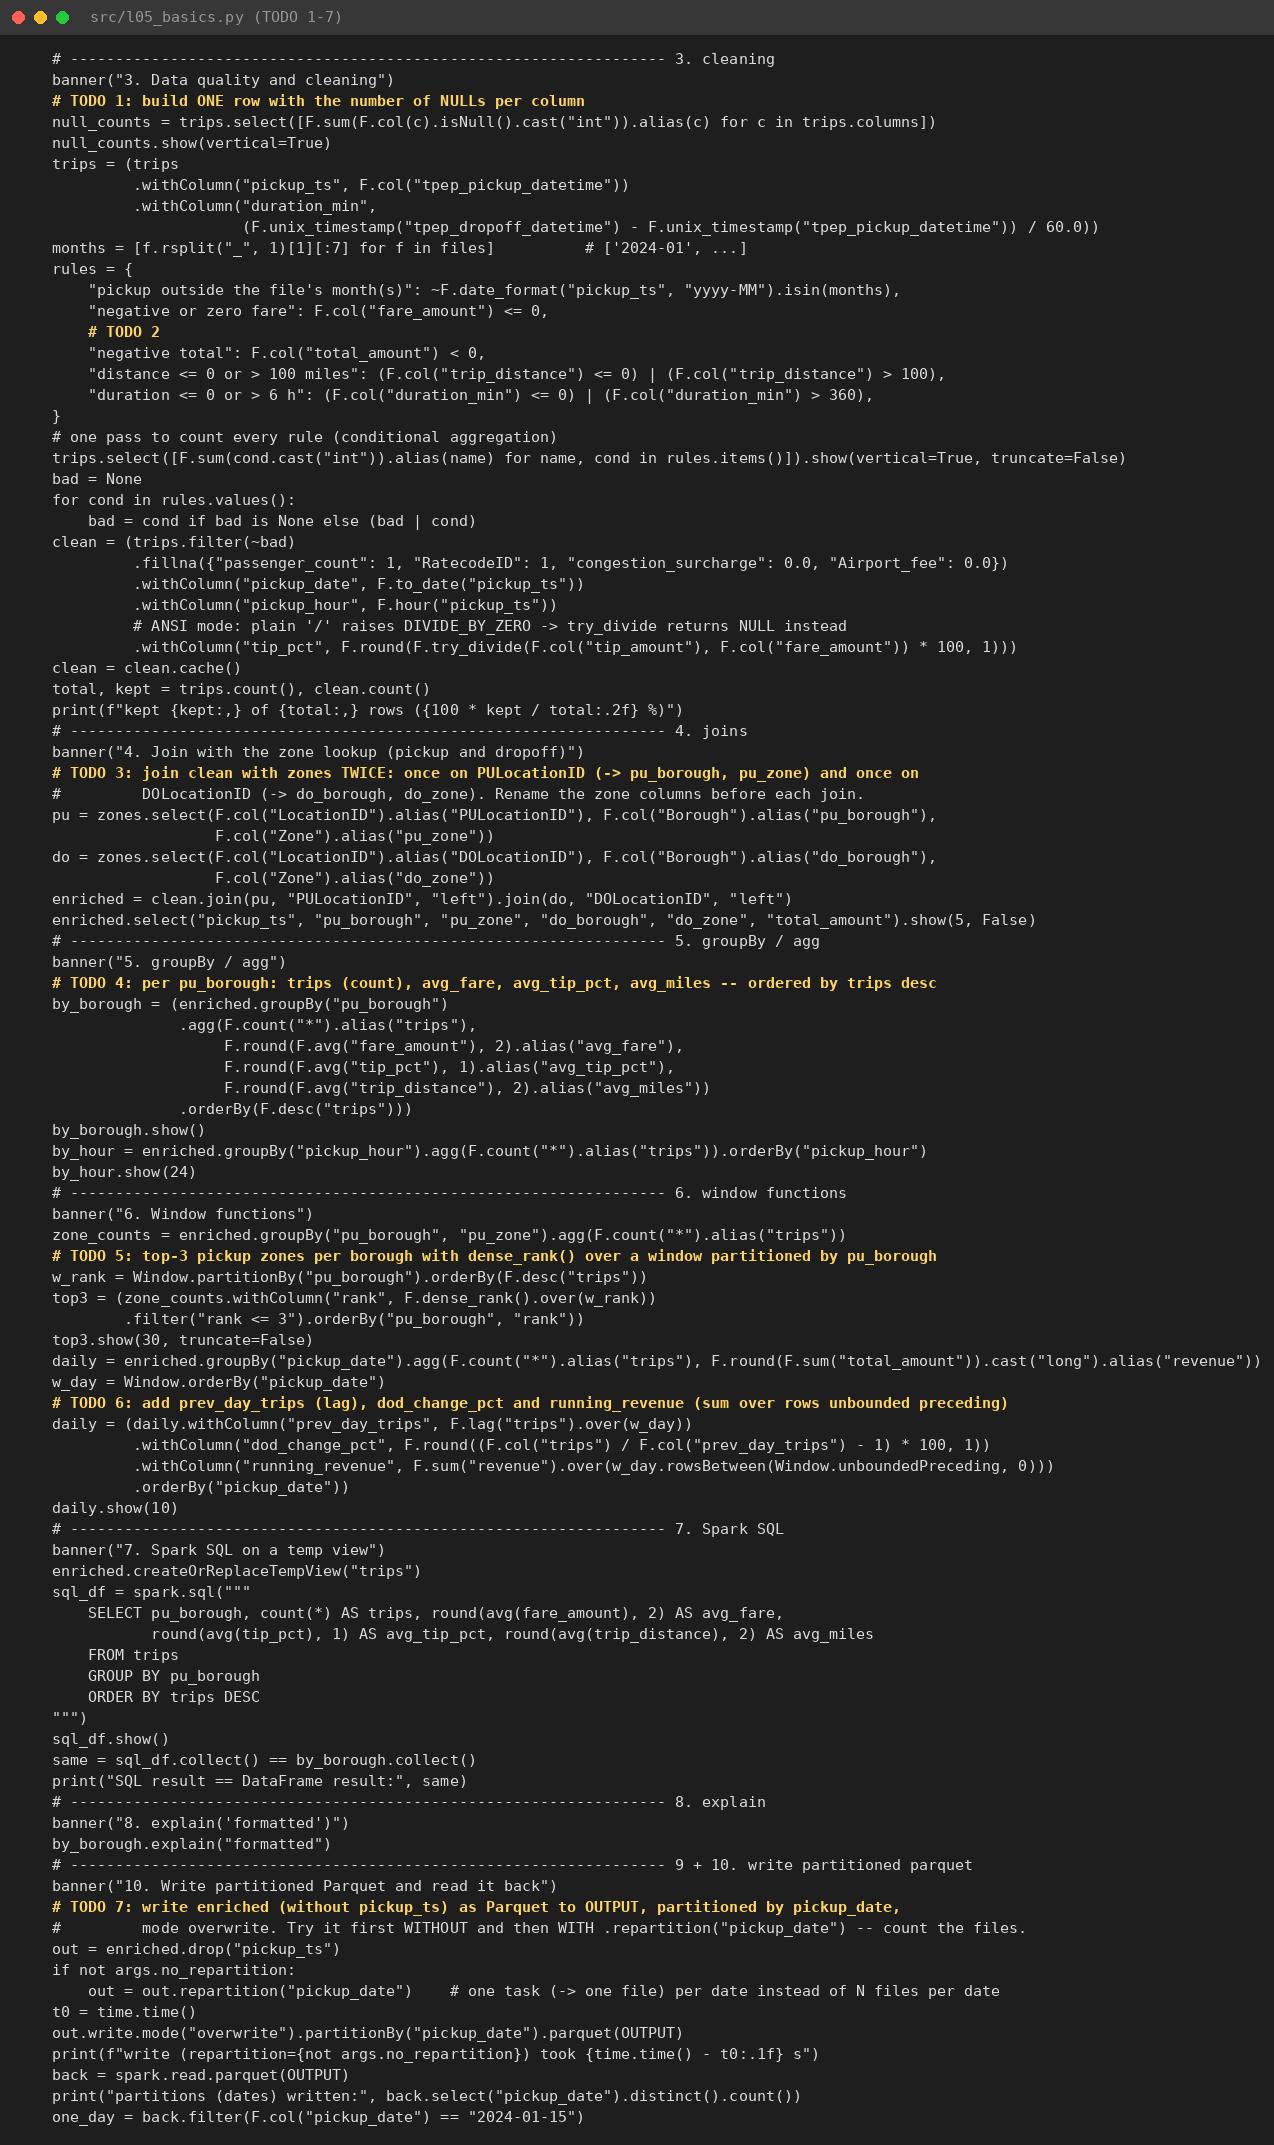
\includegraphics[keepaspectratio]{img/code_l05_basics.png}}
\caption{code}
\end{figure}

\subsection{Kết quả chính (khớp đáp
án)}\label{kux1ebft-quux1ea3-chuxednh-khux1edbp-ux111uxe1p-uxe1n}

\begin{longtable}[]{@{}
  >{\raggedright\arraybackslash}p{(\linewidth - 2\tabcolsep) * \real{0.5000}}
  >{\raggedright\arraybackslash}p{(\linewidth - 2\tabcolsep) * \real{0.5000}}@{}}
\toprule\noalign{}
\begin{minipage}[b]{\linewidth}\raggedright
Hạng mục
\end{minipage} & \begin{minipage}[b]{\linewidth}\raggedright
Kết quả
\end{minipage} \\
\midrule\noalign{}
\endhead
\bottomrule\noalign{}
\endlastfoot
Số dòng / số partition đầu vào & 2,964,624 / 4 \\
3 transformation (filter, withColumn, select) & \textbf{0.096 s}, chưa
có job nào \\
\texttt{count()} (action) & 228,254 chuyến \textgreater{} 10 dặm, 0.28
s \\
NULL ở 5 cột \texttt{passenger\_count}, \texttt{RatecodeID},
\texttt{store\_and\_fwd\_flag}, \texttt{congestion\_surcharge},
\texttt{Airport\_fee} & \textbf{140,162} mỗi cột \\
Luật làm sạch & ngoài tháng 18 · fare ≤ 0: 38,341 · total \textless{} 0:
35,504 · distance: 60,430 · duration: 2,642 \\
Giữ lại sau làm sạch & \textbf{2,867,786 / 2,964,624 (96.73 \%)} \\
Manhattan & 2,571,810 chuyến, fare 14.92, tip 21.6 \%, 2.31 dặm \\
Queens & 257,573 chuyến, fare 52.77, 12.76 dặm (sân bay) \\
Giờ đông nhất & 18:00 (206,163 chuyến) \\
Top-3 Manhattan & Midtown Center 140,065 · UES South 140,059 · UES North
133,891 \\
Top-3 Queens & JFK 138,296 · LaGuardia 87,657 · East Elmhurst 11,861 \\
SQL so với DataFrame &
\texttt{SQL\ result\ ==\ DataFrame\ result:\ True} \\
Ghi Parquet phân vùng theo ngày & 31 partition, 73 MB, 8.2 s \\
Đọc lại ngày 2024-01-15 & 74,743 chuyến, có \texttt{PartitionFilters} \\
\end{longtable}

\pandocbounded{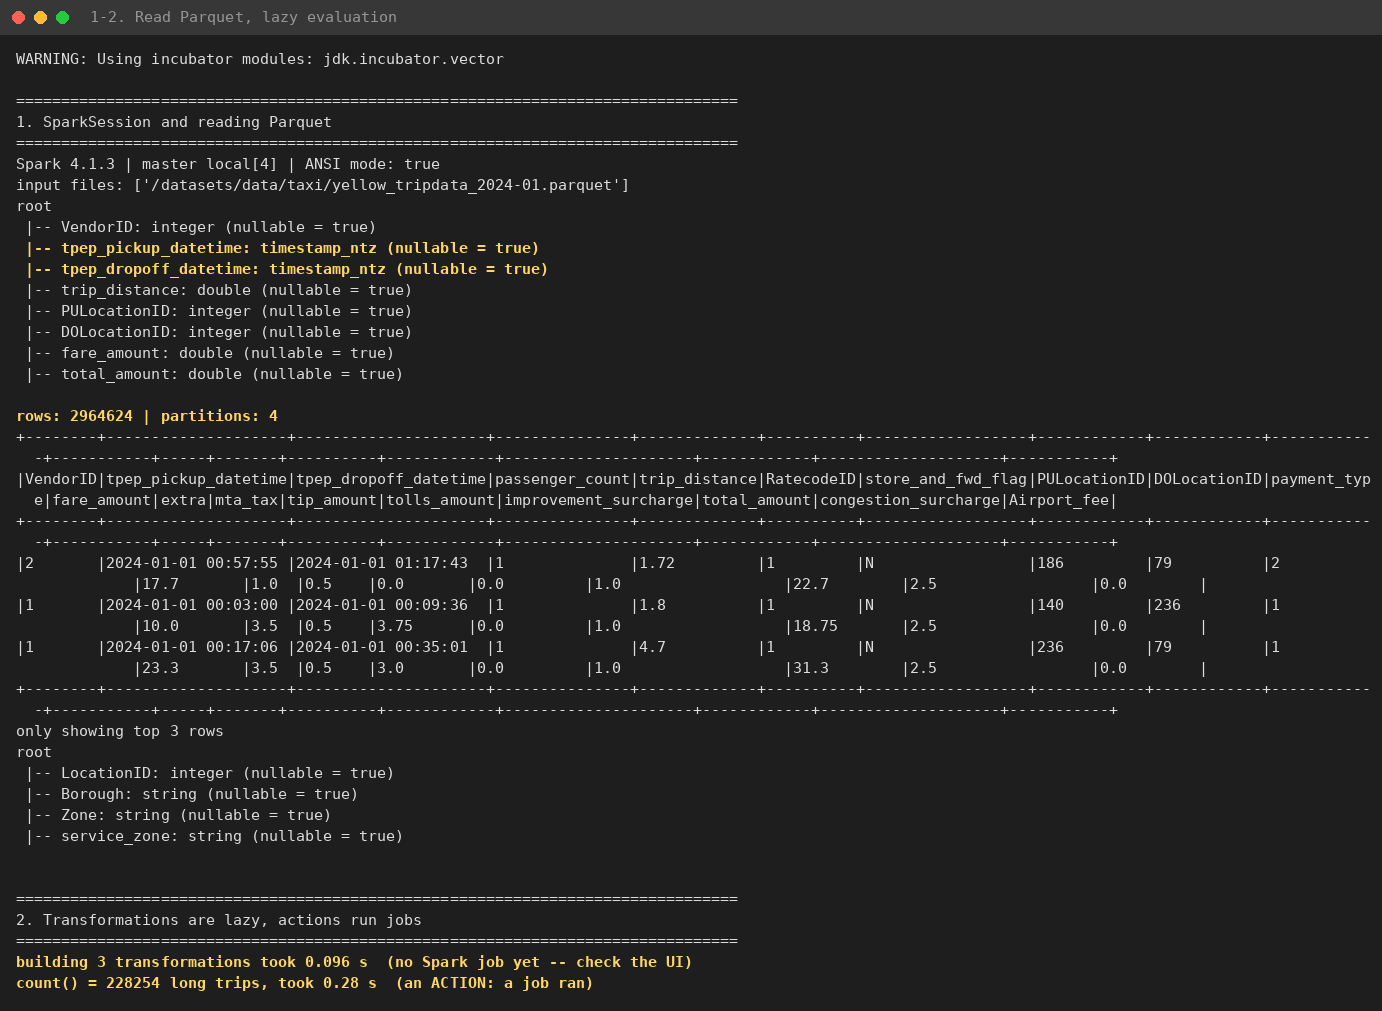
\includegraphics[keepaspectratio]{img/01_read_schema_lazy.png}}
\pandocbounded{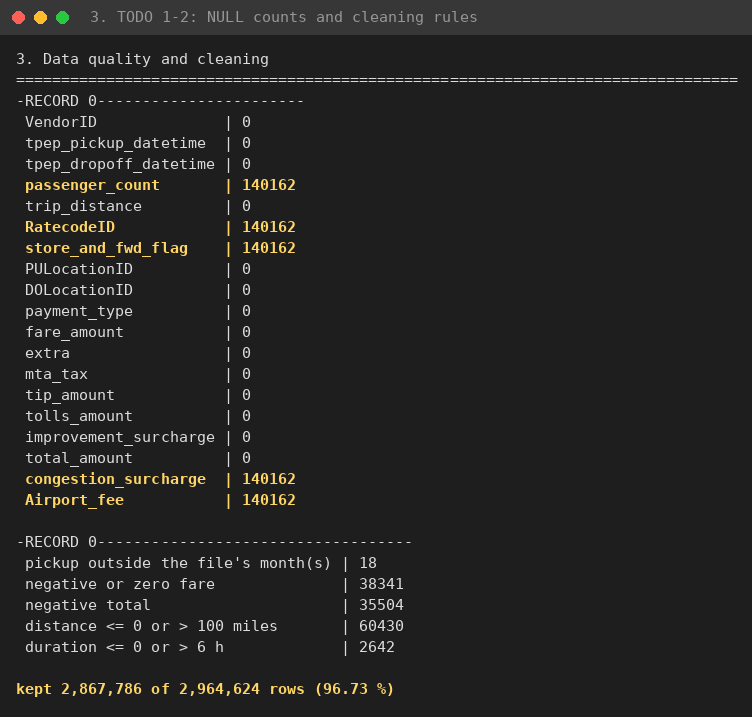
\includegraphics[keepaspectratio]{img/02_cleaning_nulls_rules.png}}
\pandocbounded{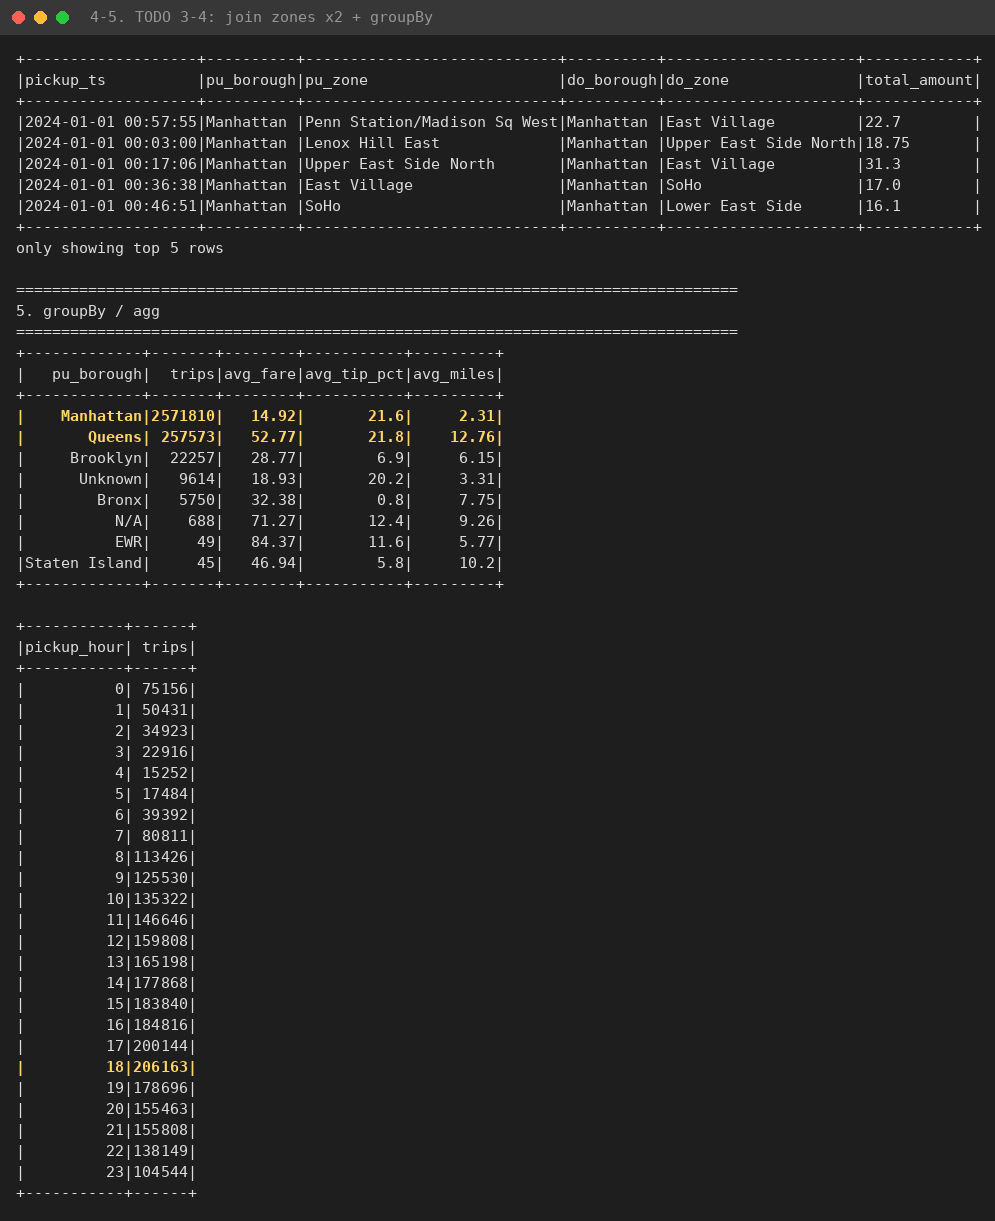
\includegraphics[keepaspectratio]{img/03_join_groupby.png}}
\pandocbounded{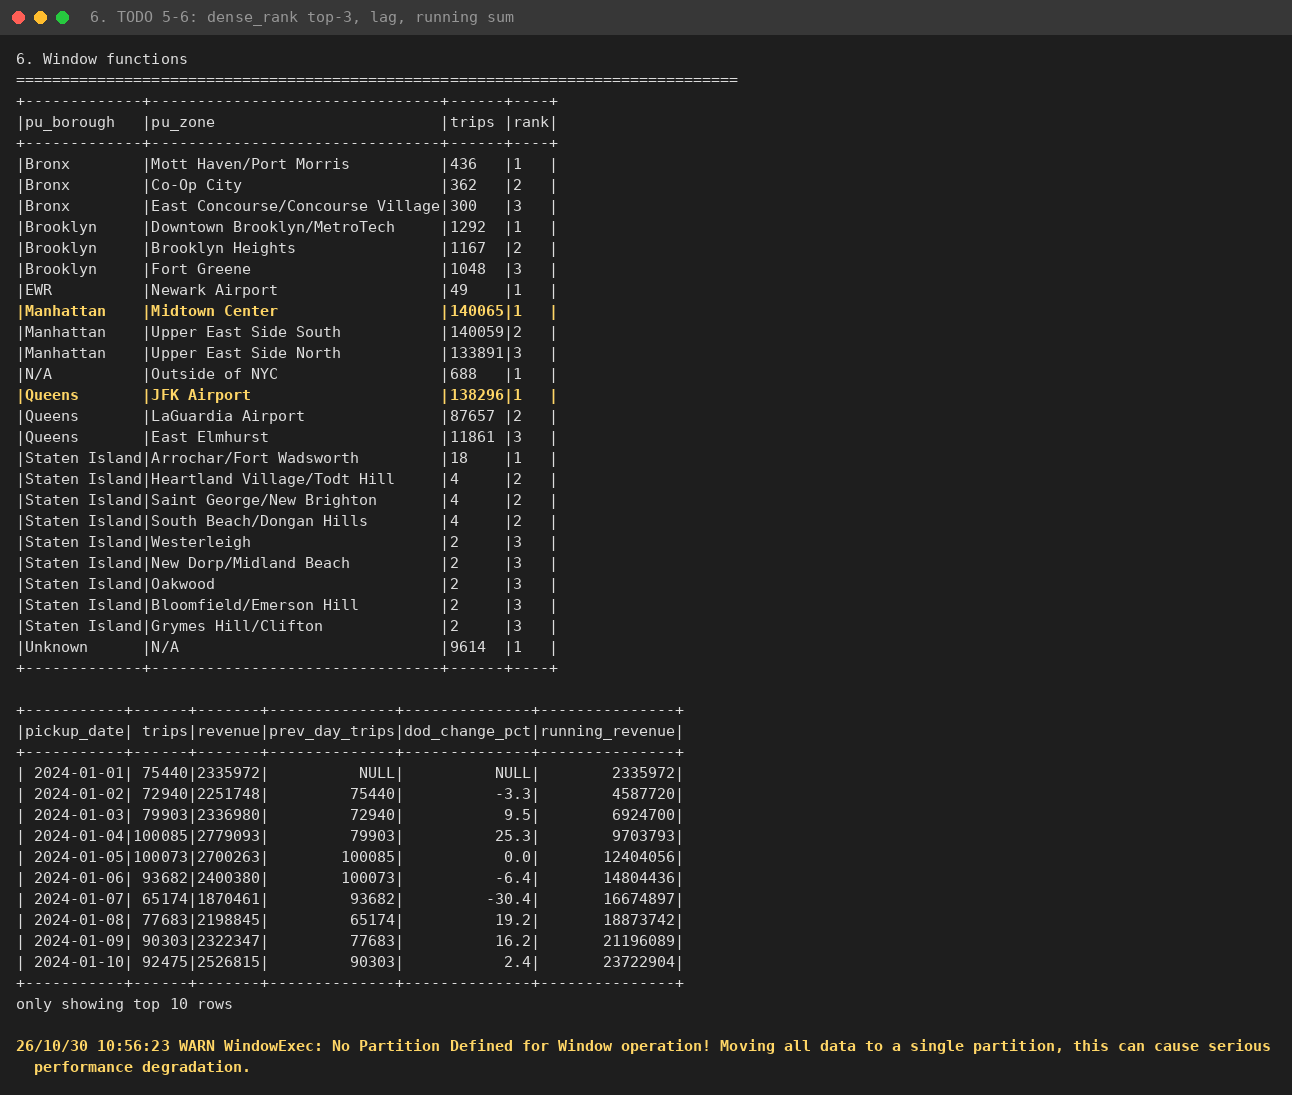
\includegraphics[keepaspectratio]{img/04_window_functions.png}}

Spark 4 bật \textbf{ANSI mode} mặc định: \texttt{1/0} báo lỗi
\texttt{{[}DIVIDE\_BY\_ZERO{]}} thay vì trả NULL. Vì vậy script tính
\texttt{tip\_pct} bằng \texttt{F.try\_divide}.

\begin{figure}
\centering
\pandocbounded{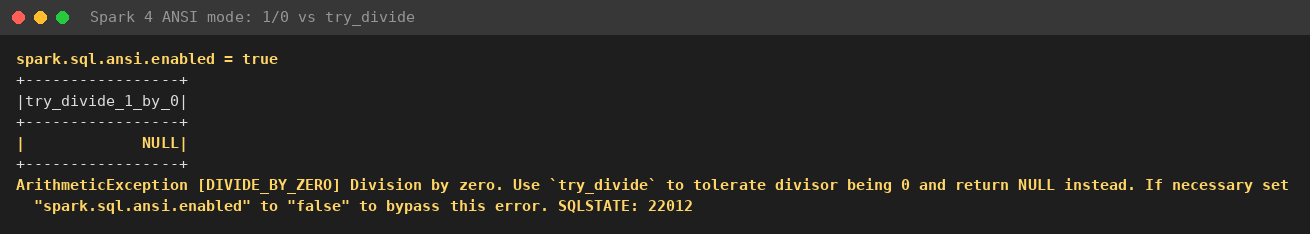
\includegraphics[keepaspectratio]{img/08_ansi_divide_by_zero.png}}
\caption{ansi}
\end{figure}

\subsection{Plan và Spark UI}\label{plan-vuxe0-spark-ui}

\pandocbounded{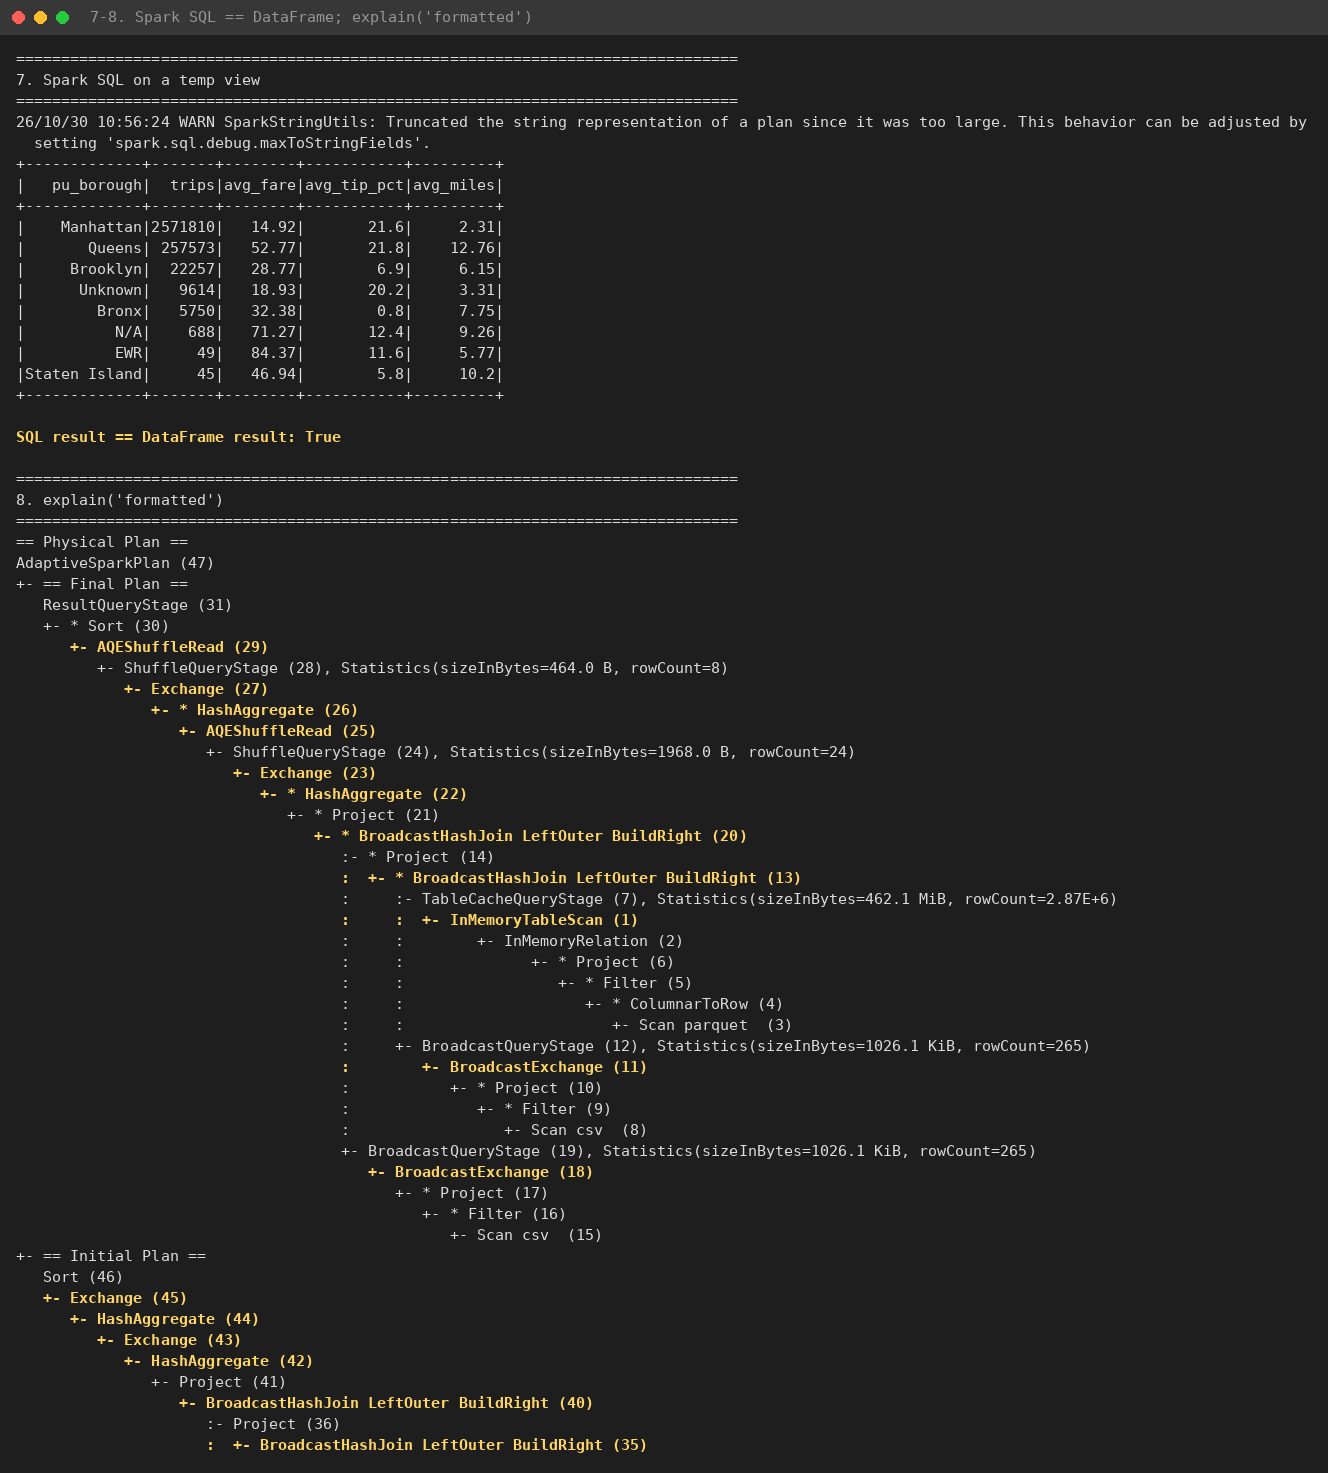
\includegraphics[keepaspectratio]{img/05_sql_and_plan_tree.png}}
\pandocbounded{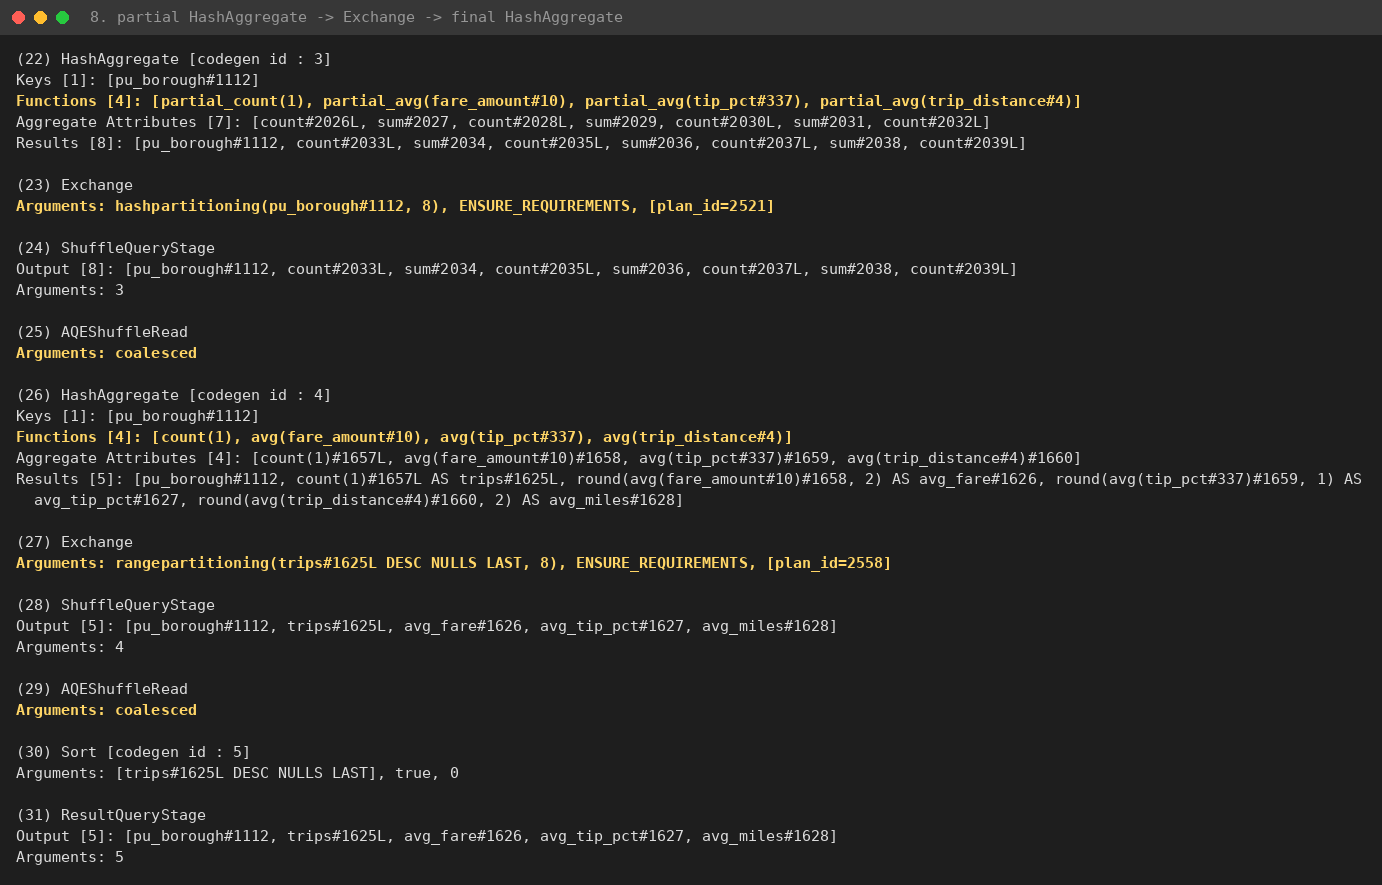
\includegraphics[keepaspectratio]{img/06_plan_partial_final_agg.png}}

\begin{longtable}[]{@{}
  >{\raggedright\arraybackslash}p{(\linewidth - 4\tabcolsep) * \real{0.3333}}
  >{\raggedright\arraybackslash}p{(\linewidth - 4\tabcolsep) * \real{0.3333}}
  >{\raggedright\arraybackslash}p{(\linewidth - 4\tabcolsep) * \real{0.3333}}@{}}
\toprule\noalign{}
\begin{minipage}[b]{\linewidth}\raggedright
Tab
\end{minipage} & \begin{minipage}[b]{\linewidth}\raggedright
Ảnh
\end{minipage} & \begin{minipage}[b]{\linewidth}\raggedright
Nhận xét
\end{minipage} \\
\midrule\noalign{}
\endhead
\bottomrule\noalign{}
\endlastfoot
Jobs &
\pandocbounded{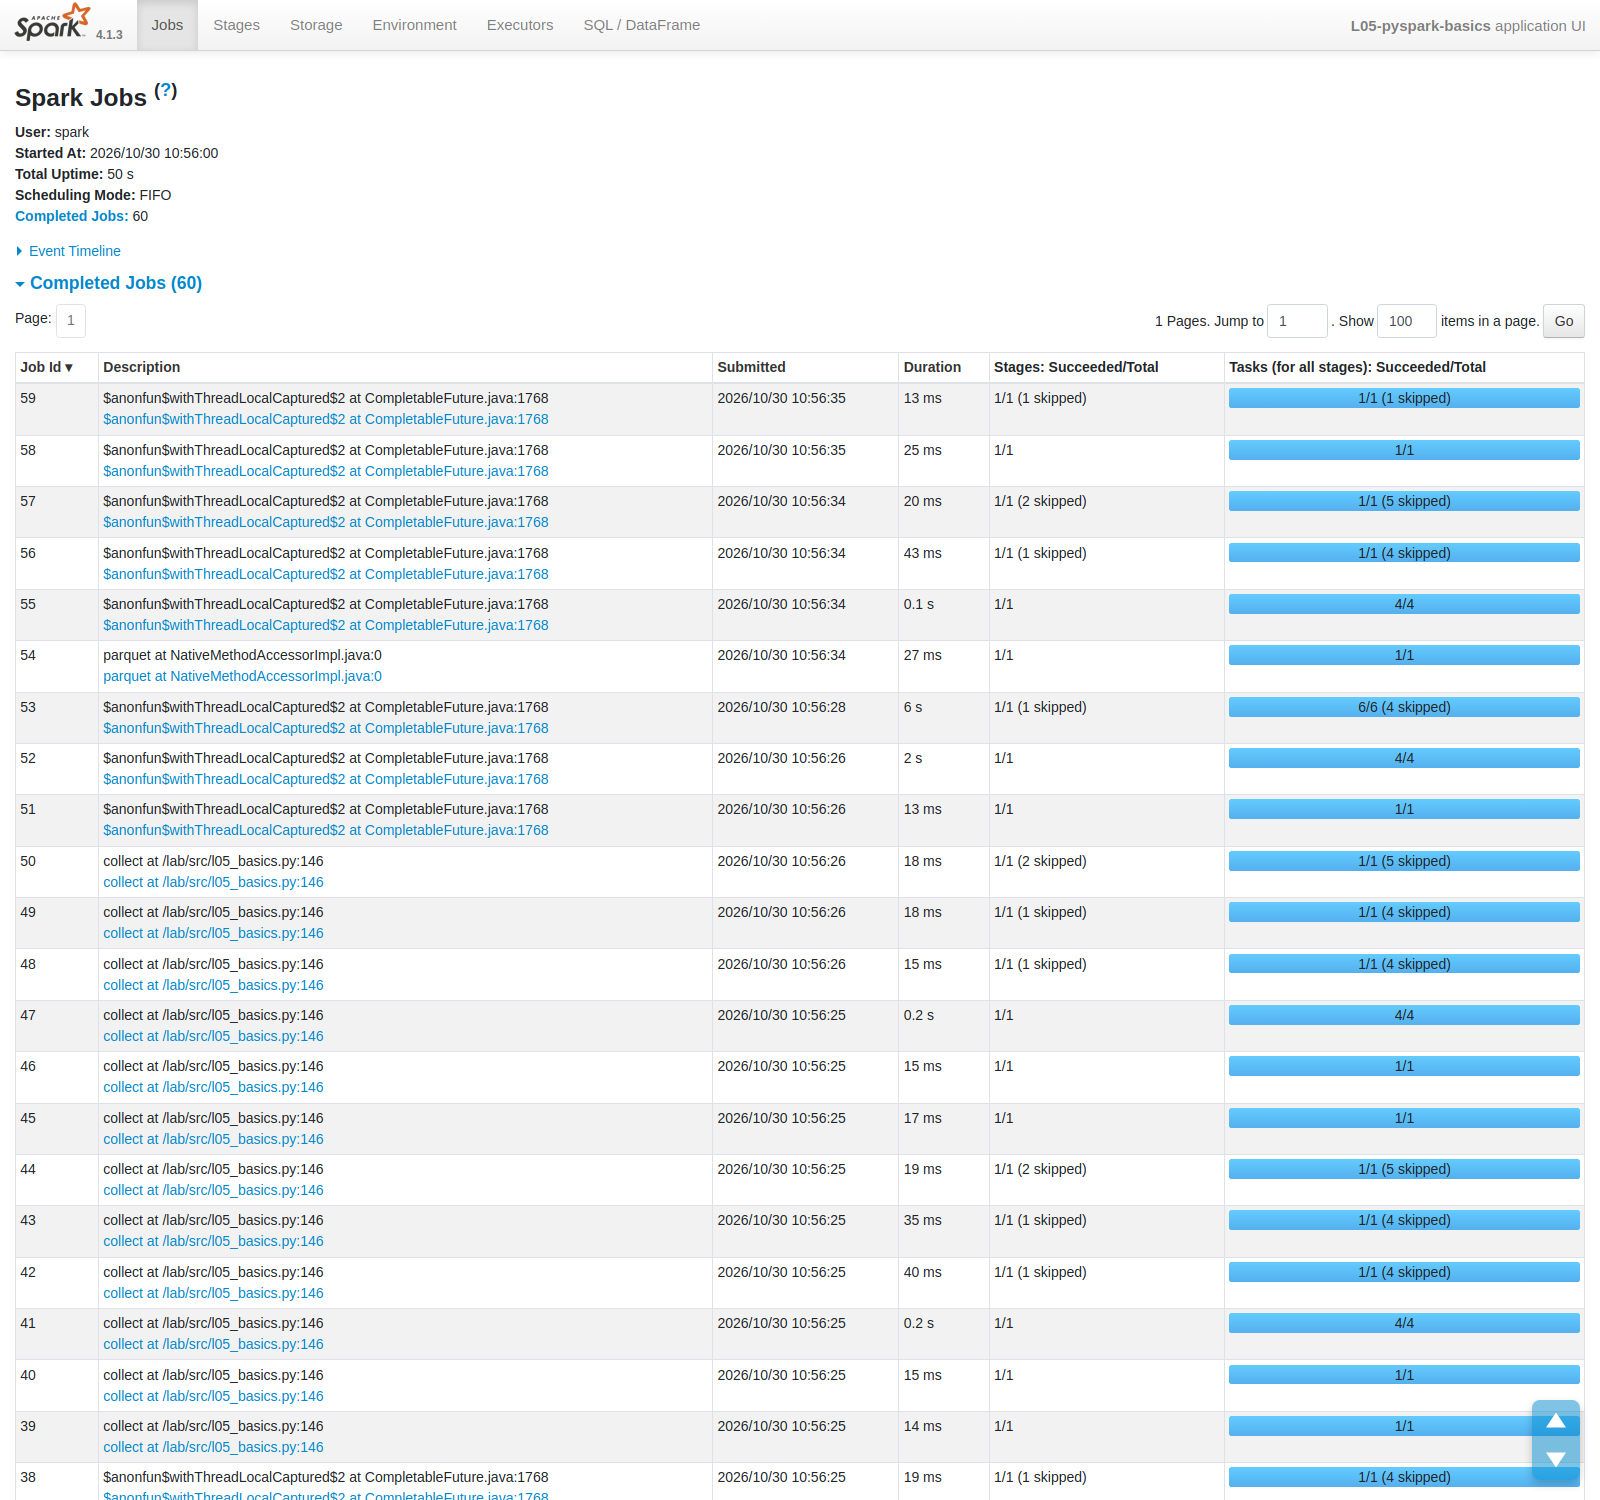
\includegraphics[keepaspectratio]{img/20_ui_jobs.png}} &
mỗi action (\texttt{count}, \texttt{showString}, \texttt{collect},
\texttt{parquet}) sinh ra một hoặc nhiều job \\
Stages &
\pandocbounded{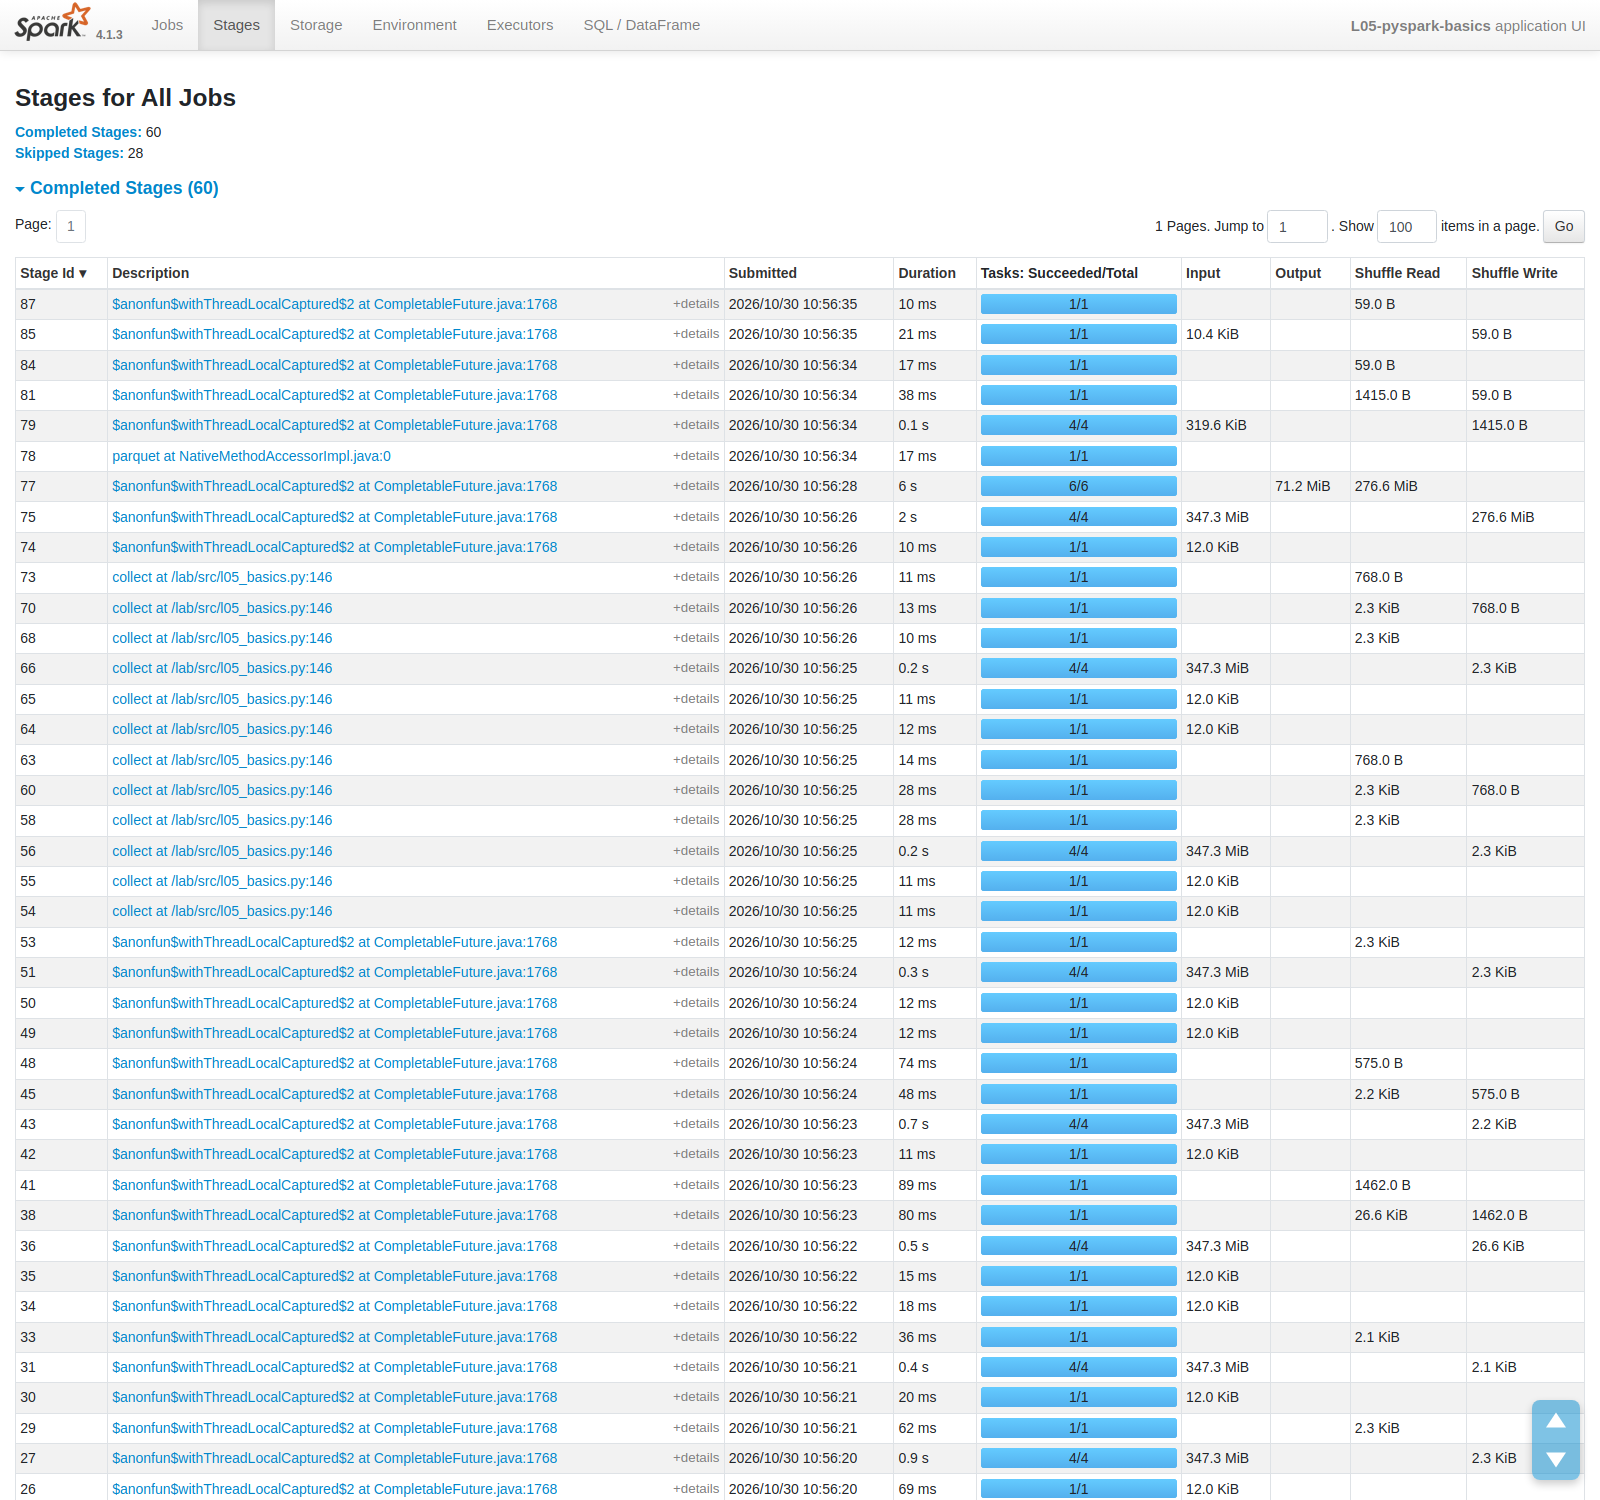
\includegraphics[keepaspectratio]{img/21_ui_stages.png}}
& có cột Shuffle Read/Write; stage 4 task đọc từ cache \\
Storage &
\pandocbounded{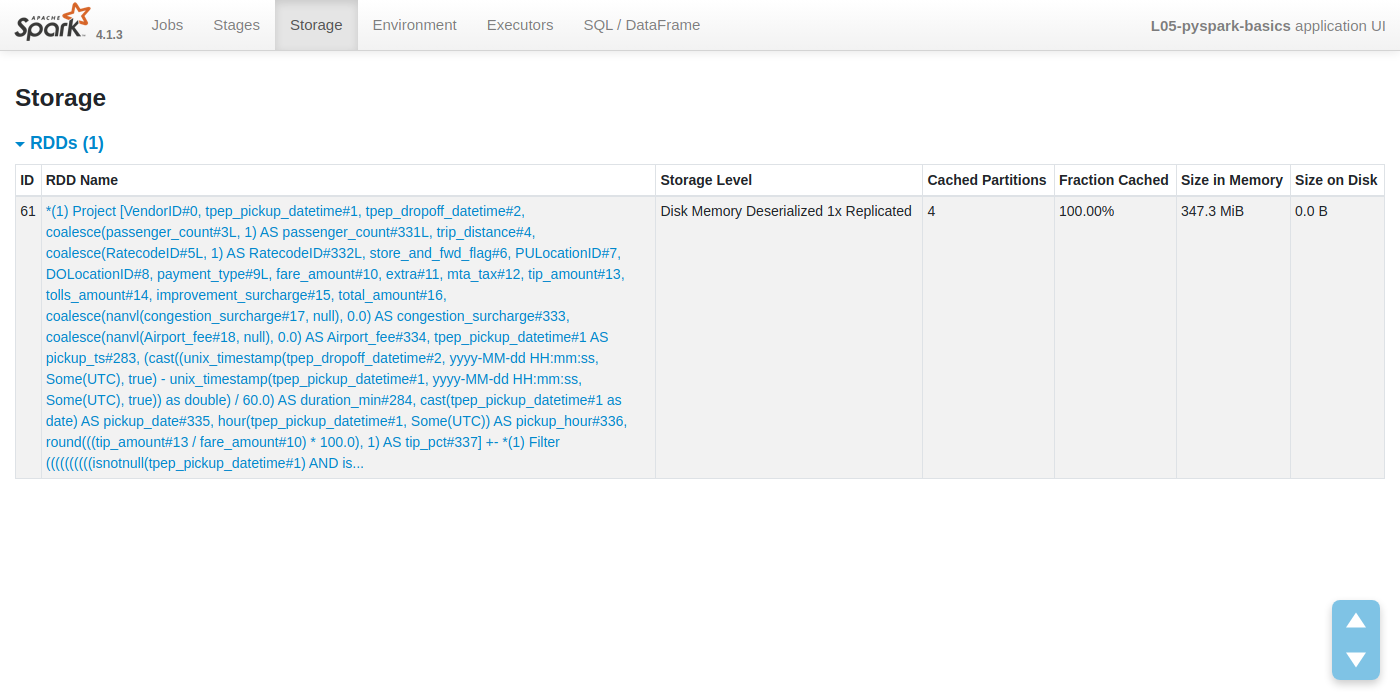
\includegraphics[keepaspectratio]{img/22_ui_storage_cache.png}}
& DataFrame \texttt{clean} được cache: 4/4 partition, \textbf{100 \%},
\textbf{347.3 MiB} trong bộ nhớ \\
SQL (query 10 = \texttt{by\_borough.show()}) &
\pandocbounded{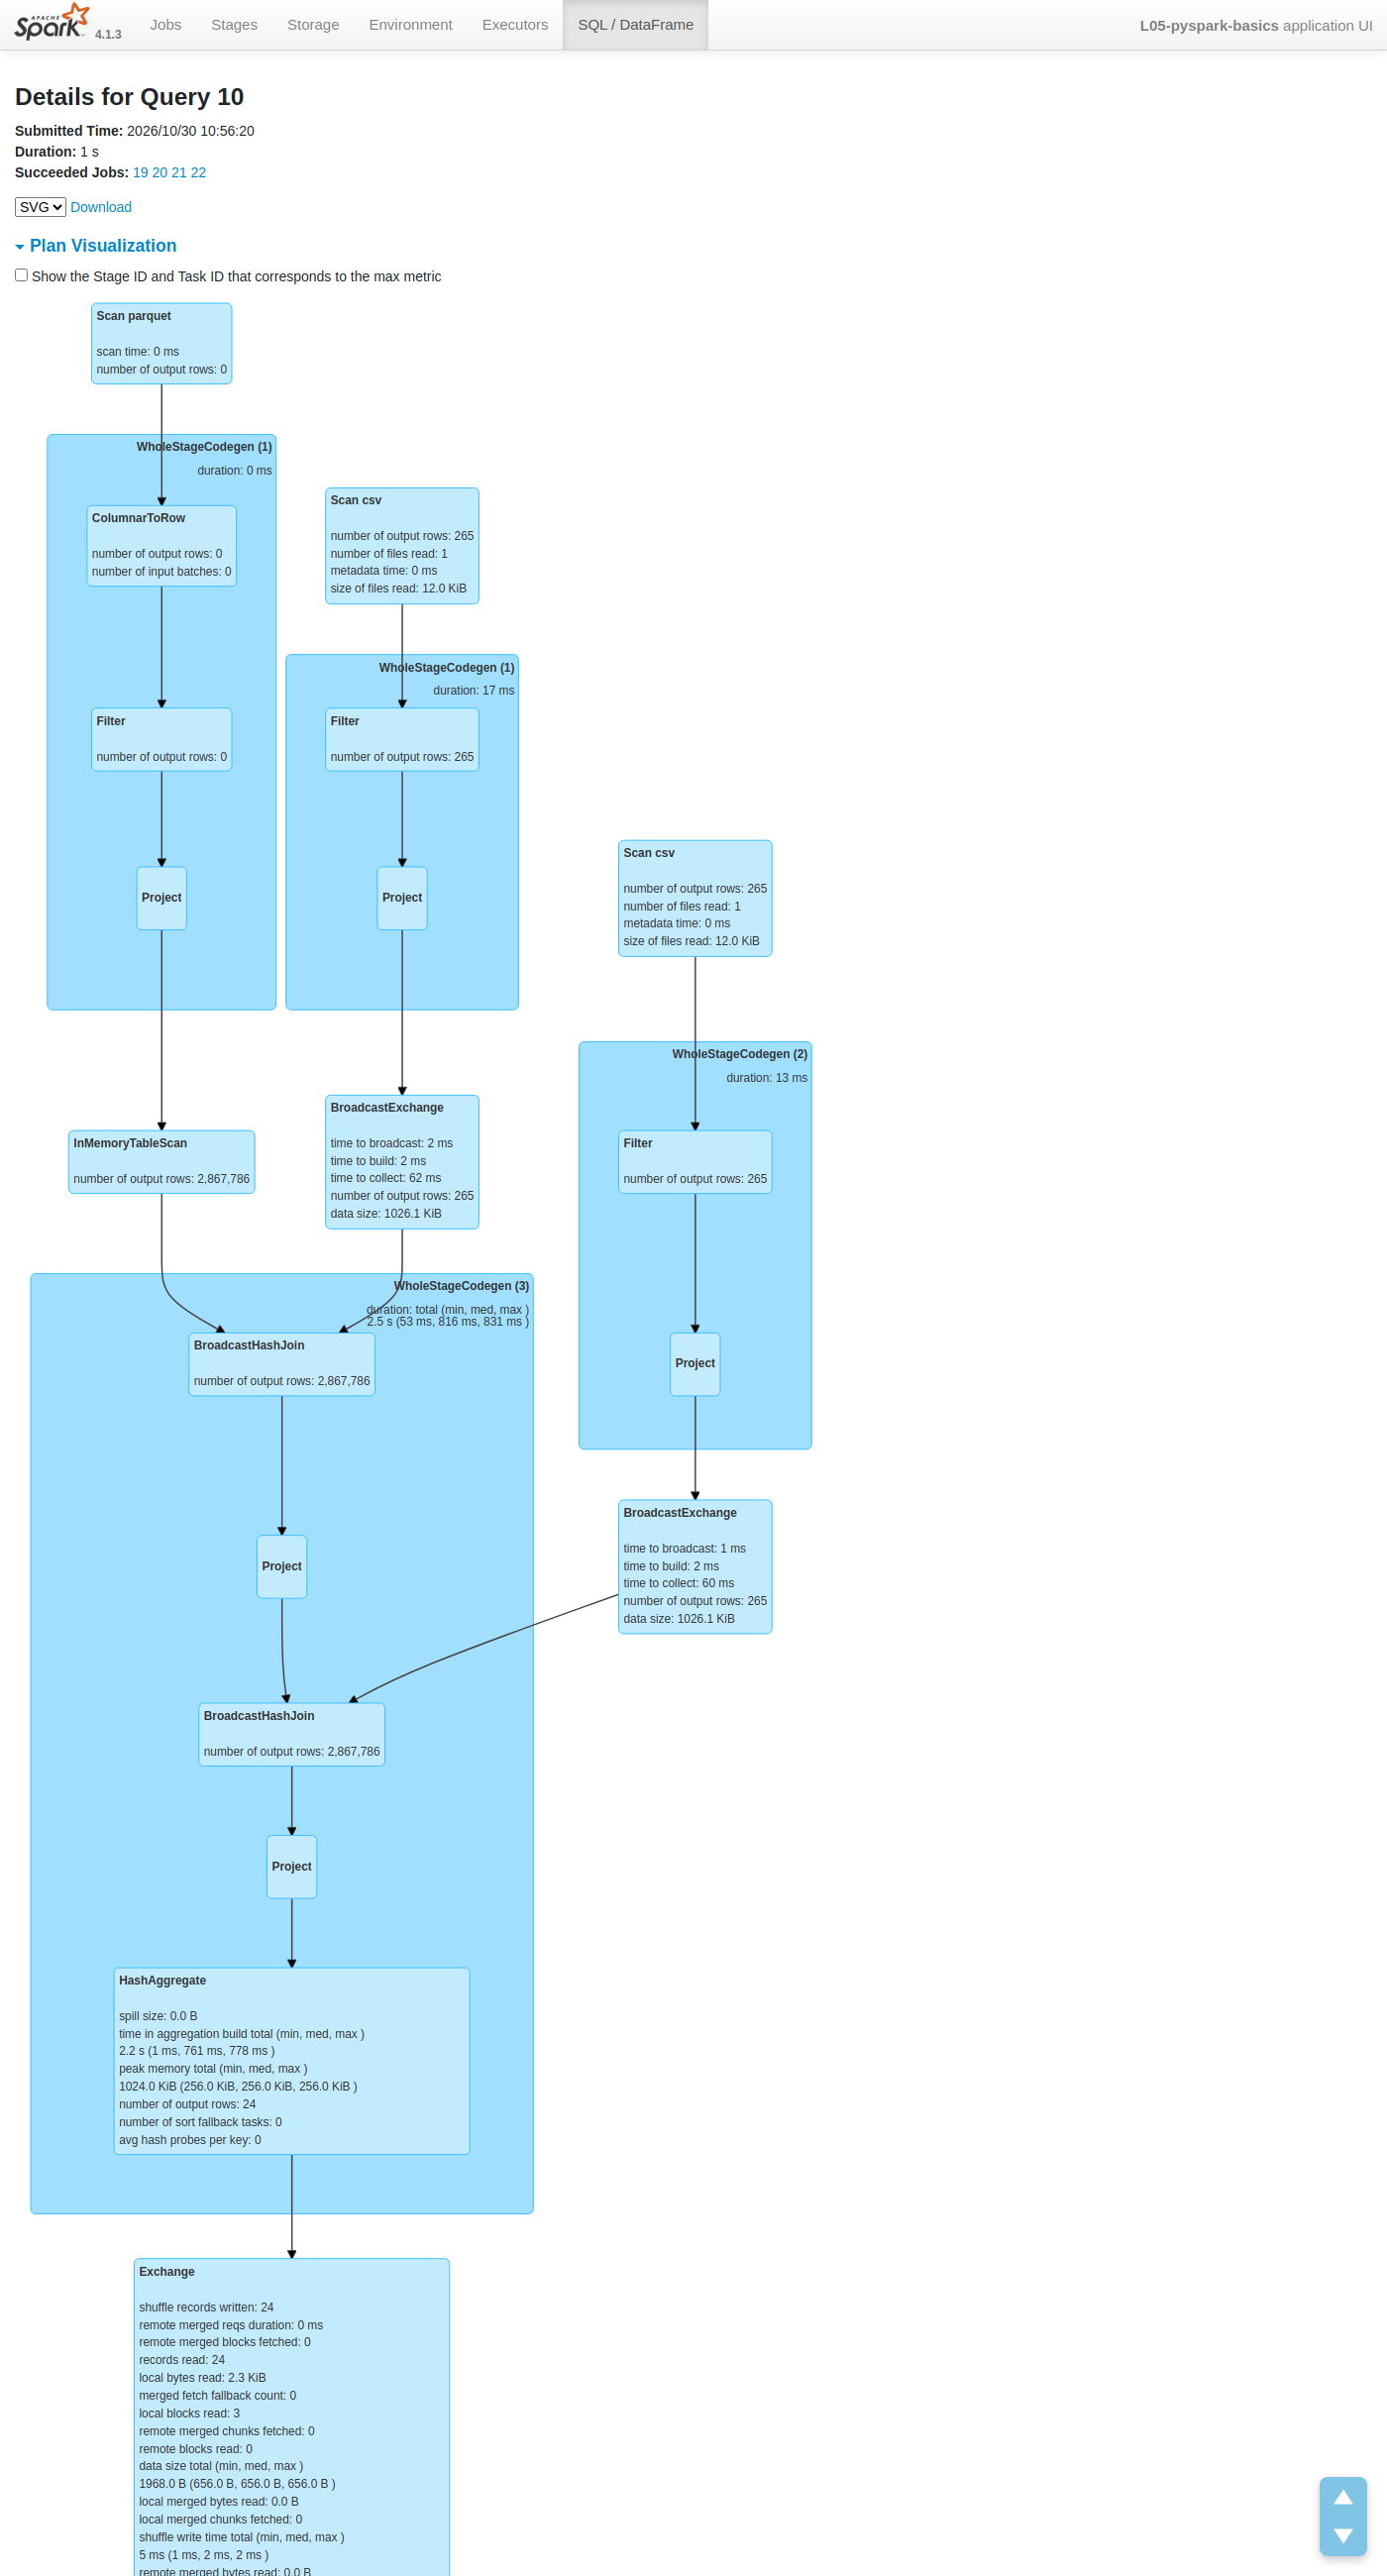
\includegraphics[keepaspectratio]{img/24_ui_sql_by_borough_plan.png}}
& \texttt{InMemoryTableScan} 2,867,786 dòng → 2 ×
\texttt{BroadcastHashJoin} (265 dòng) → \texttt{HashAggregate} partial:
\textbf{24 dòng} → \texttt{Exchange} \\
Job 22 &
\pandocbounded{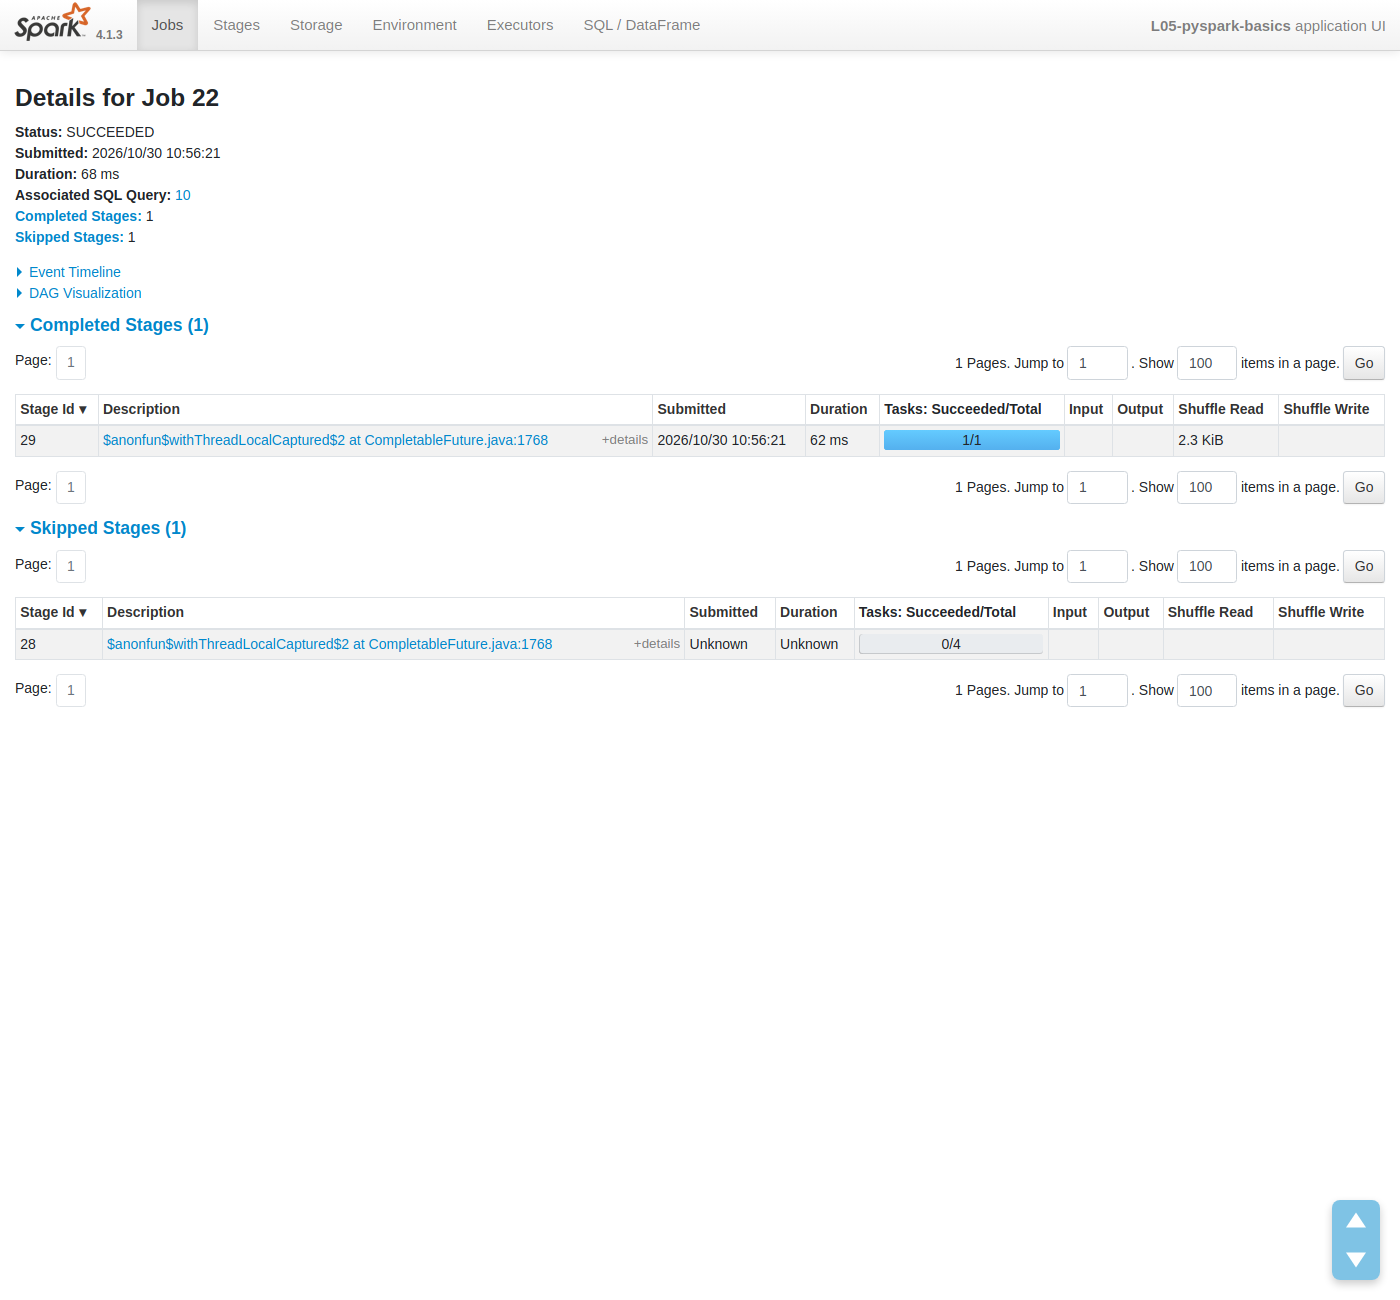
\includegraphics[keepaspectratio]{img/28_ui_job22_dag.png}}
& stage 28 \emph{skipped} (dùng lại shuffle của job 21); stage 29 chạy 1
task, Shuffle Read 2.3 KiB \\
Khác &
\pandocbounded{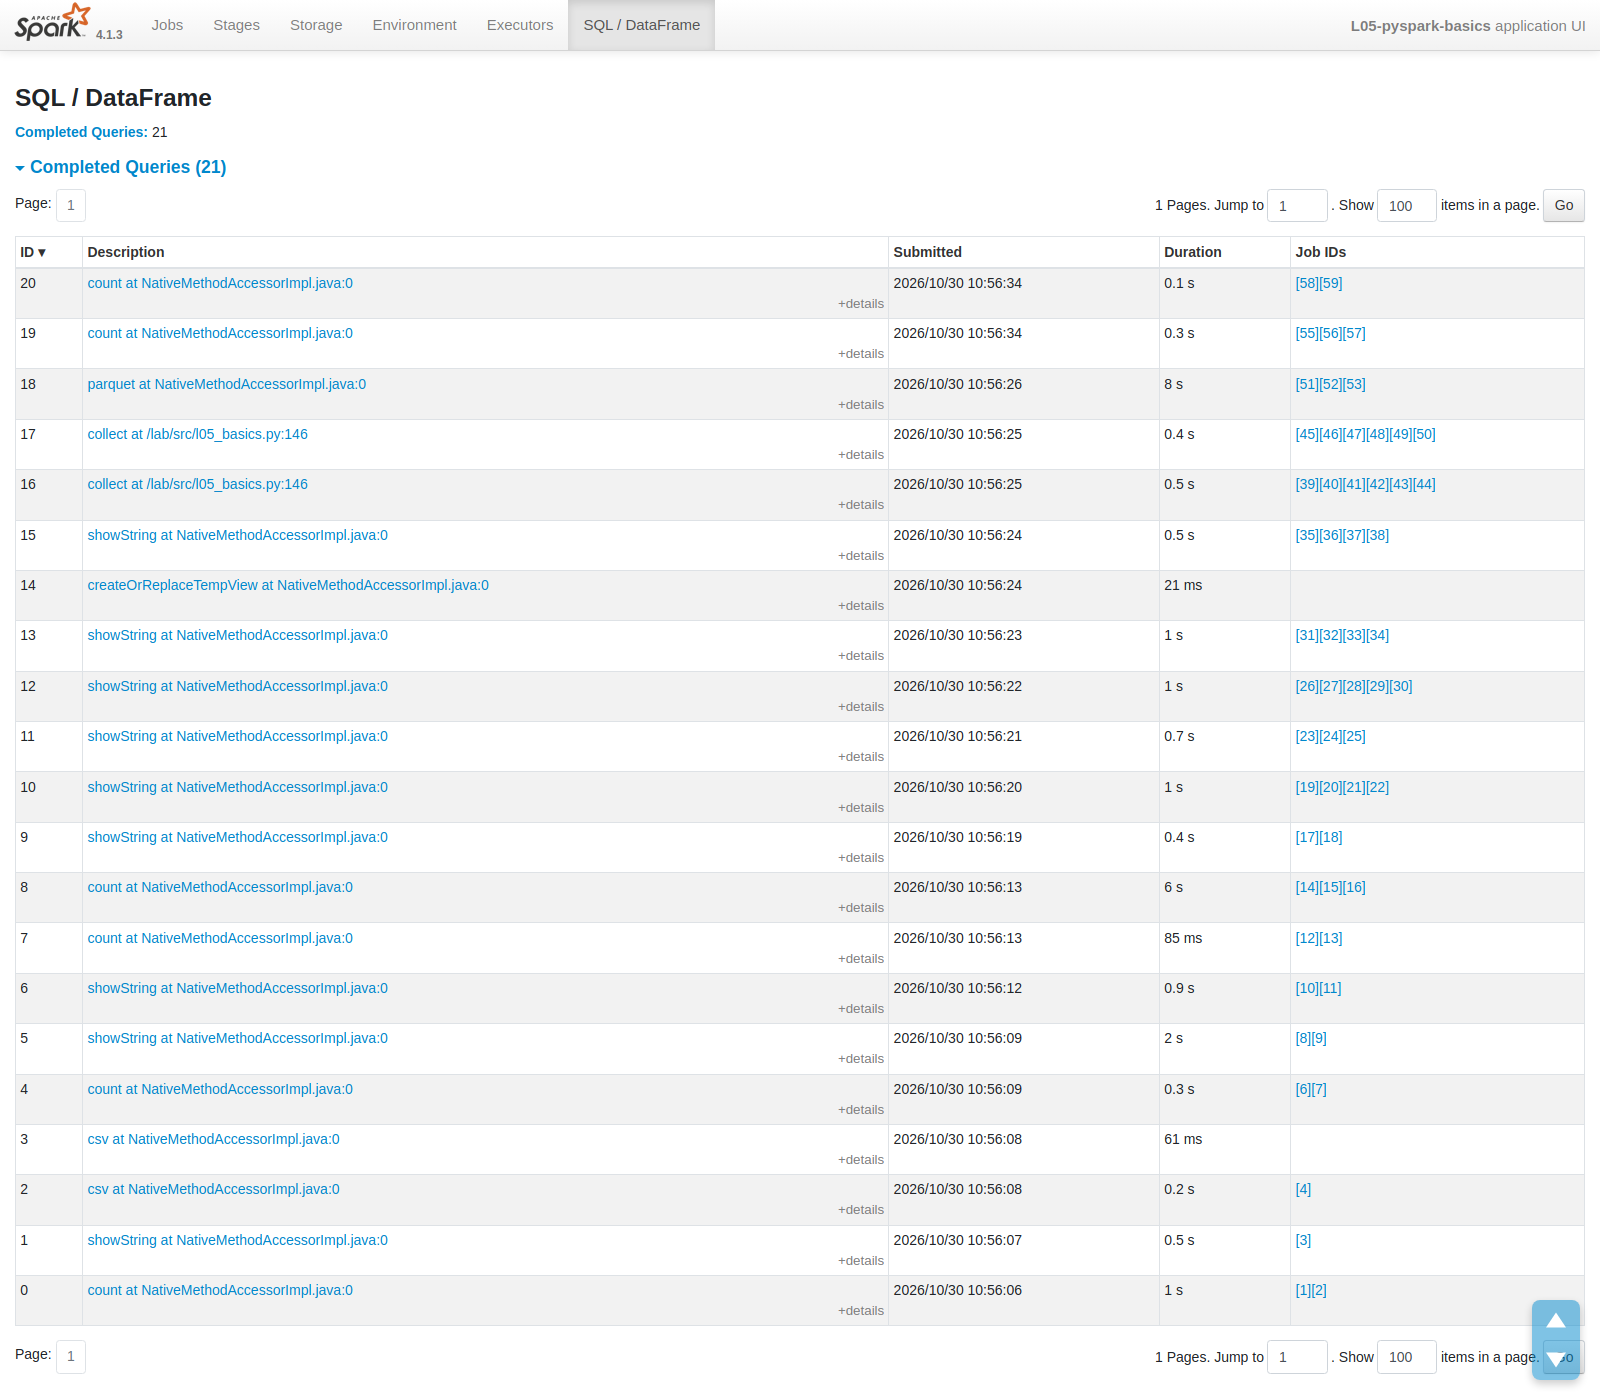
\includegraphics[keepaspectratio]{img/23_ui_sql_list.png}}
\pandocbounded{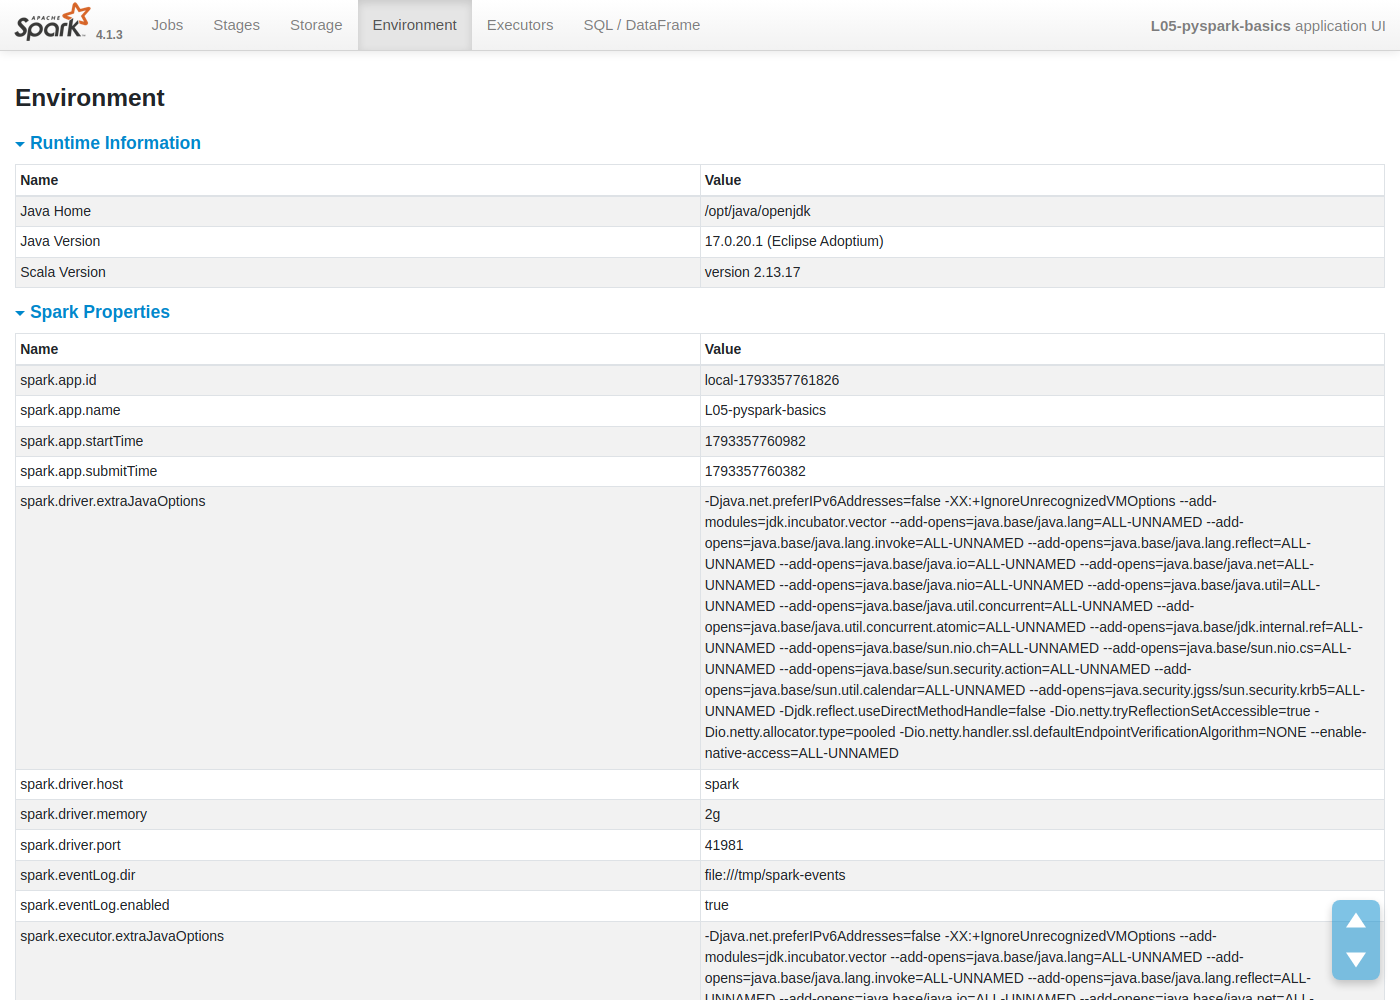
\includegraphics[keepaspectratio]{img/25_ui_environment.png}}
\pandocbounded{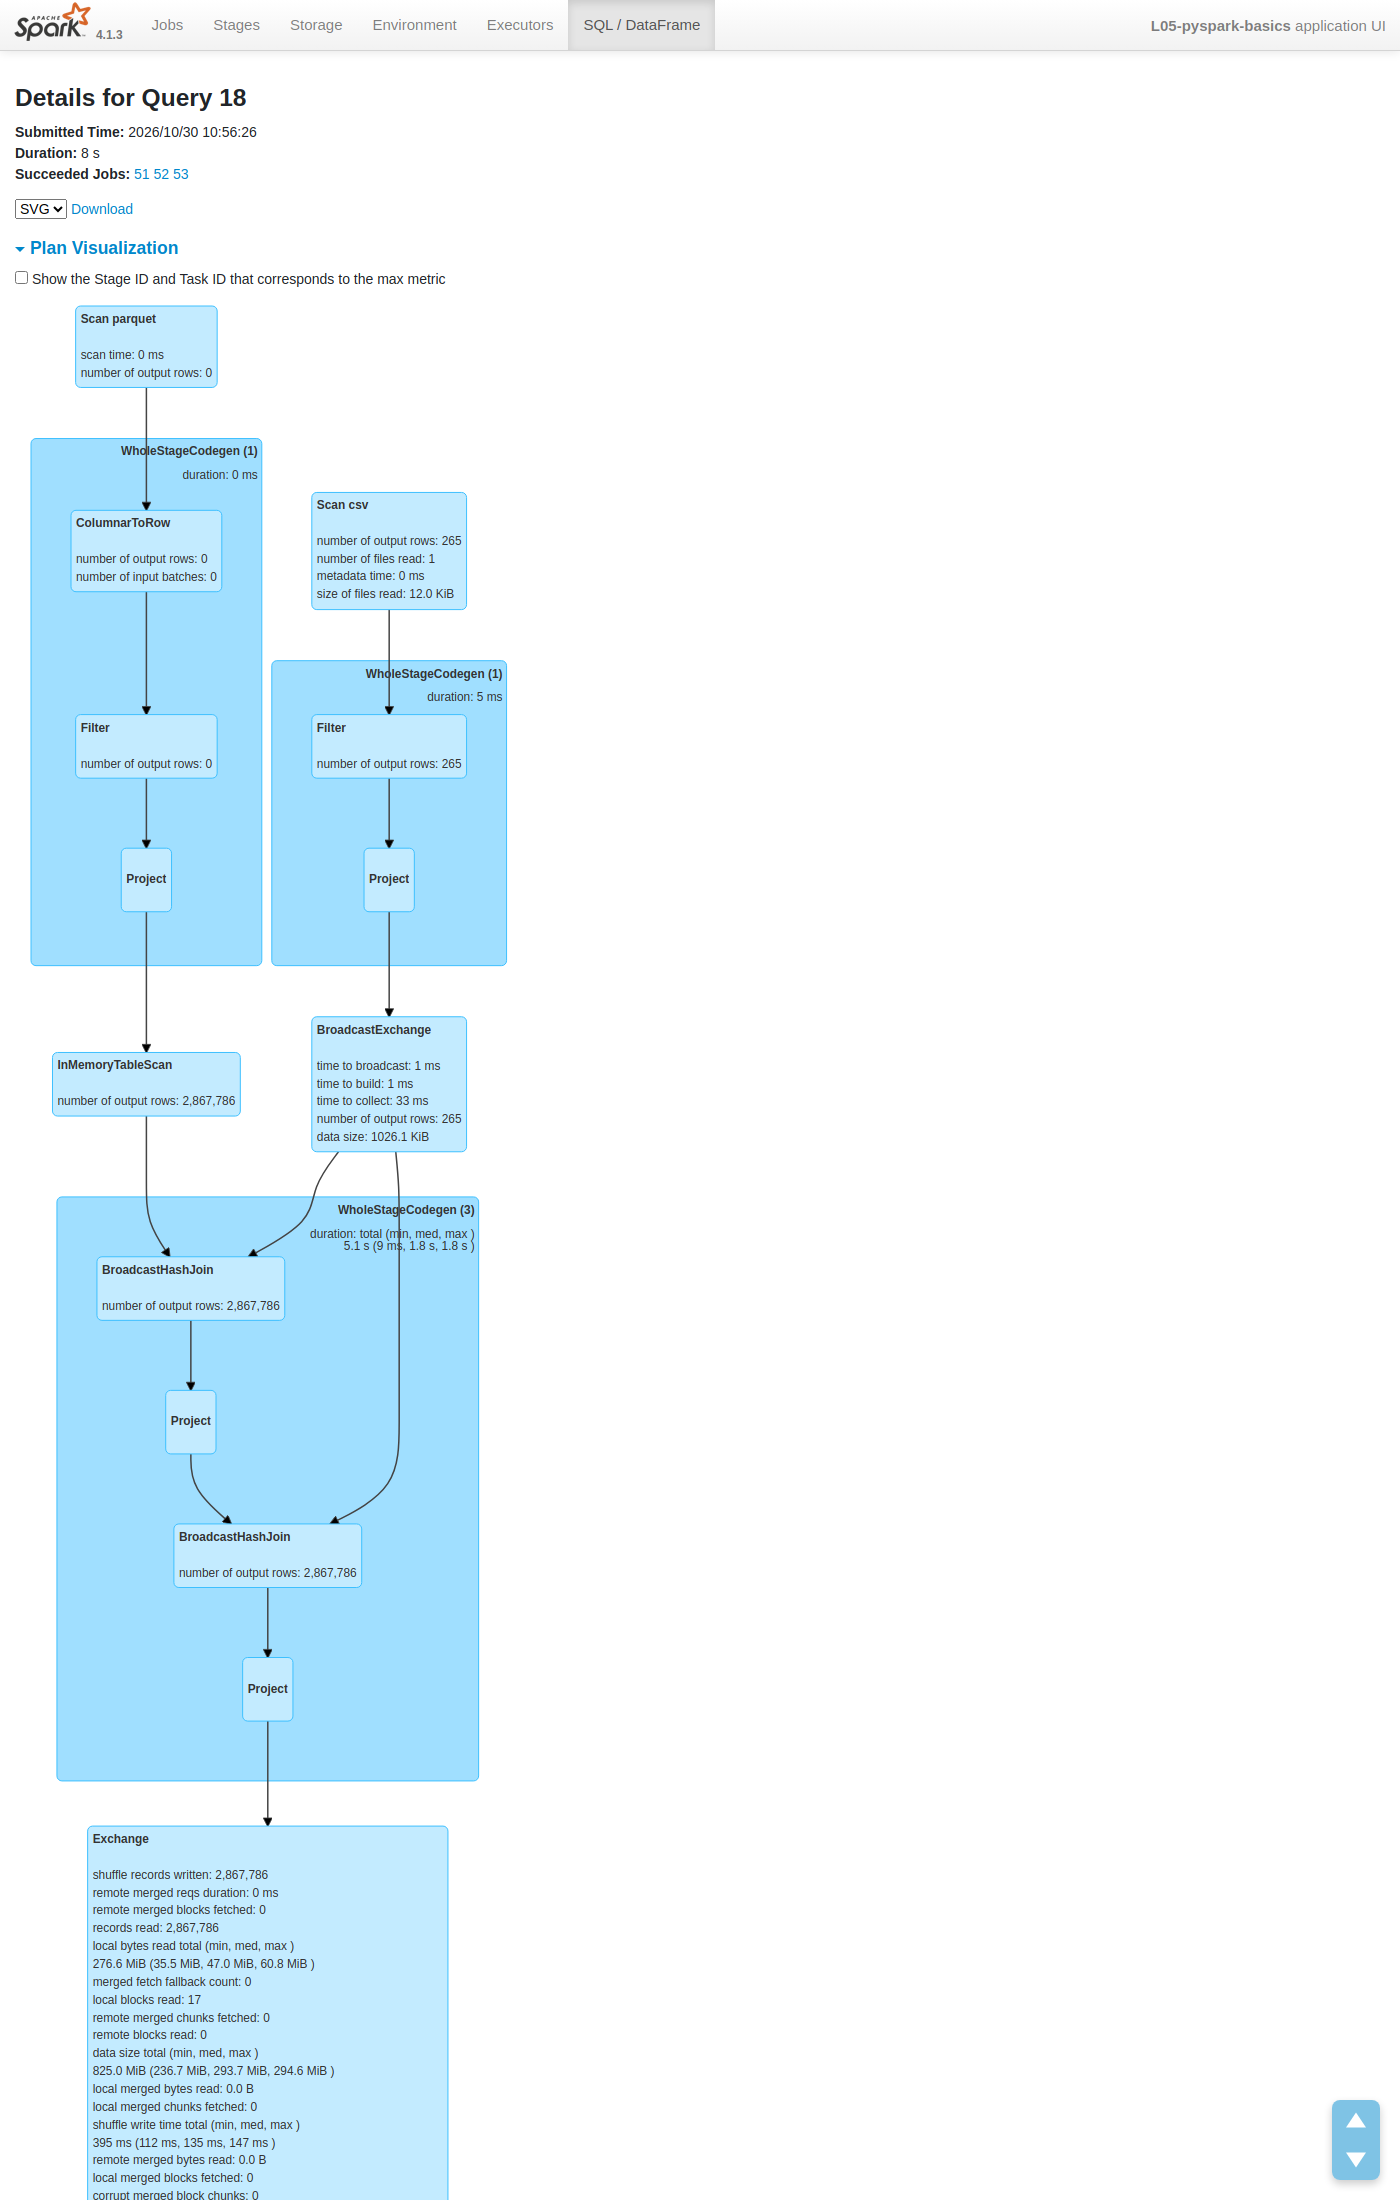
\includegraphics[keepaspectratio]{img/26_ui_sql_write_parquet.png}}
\pandocbounded{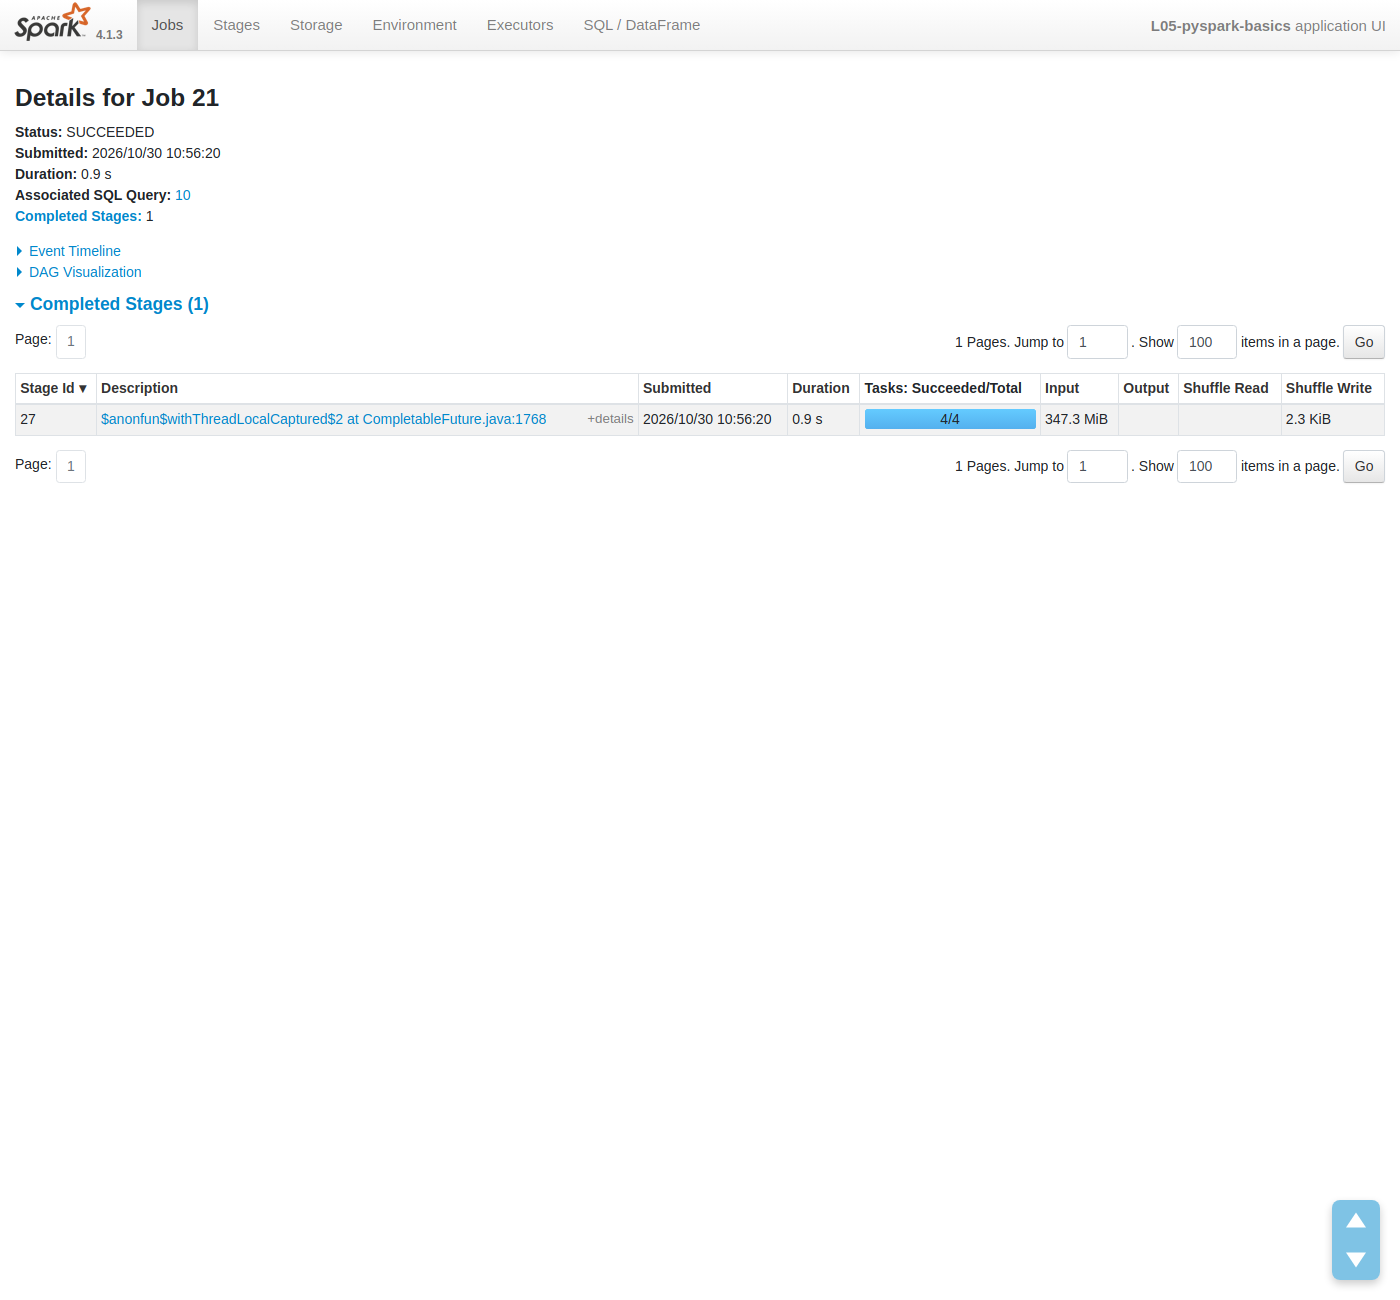
\includegraphics[keepaspectratio]{img/27_ui_job21_dag.png}}
& \\
\end{longtable}

\subsection{Ghi Parquet phân vùng (TODO
7)}\label{ghi-parquet-phuxe2n-vuxf9ng-todo-7}

\begin{longtable}[]{@{}lll@{}}
\toprule\noalign{}
& Không \texttt{repartition} & \texttt{repartition("pickup\_date")} \\
\midrule\noalign{}
\endhead
\bottomrule\noalign{}
\endlastfoot
Số file \texttt{.parquet} & \textbf{56} & \textbf{31} (1 file/ngày) \\
File trong \texttt{pickup\_date=2024-01-15} & 2 & 1 \\
Dung lượng & 74 MB & 73 MB \\
Thời gian ghi & 6.8 s & 8.2 s (thêm 1 shuffle) \\
\end{longtable}

\begin{figure}
\centering
\pandocbounded{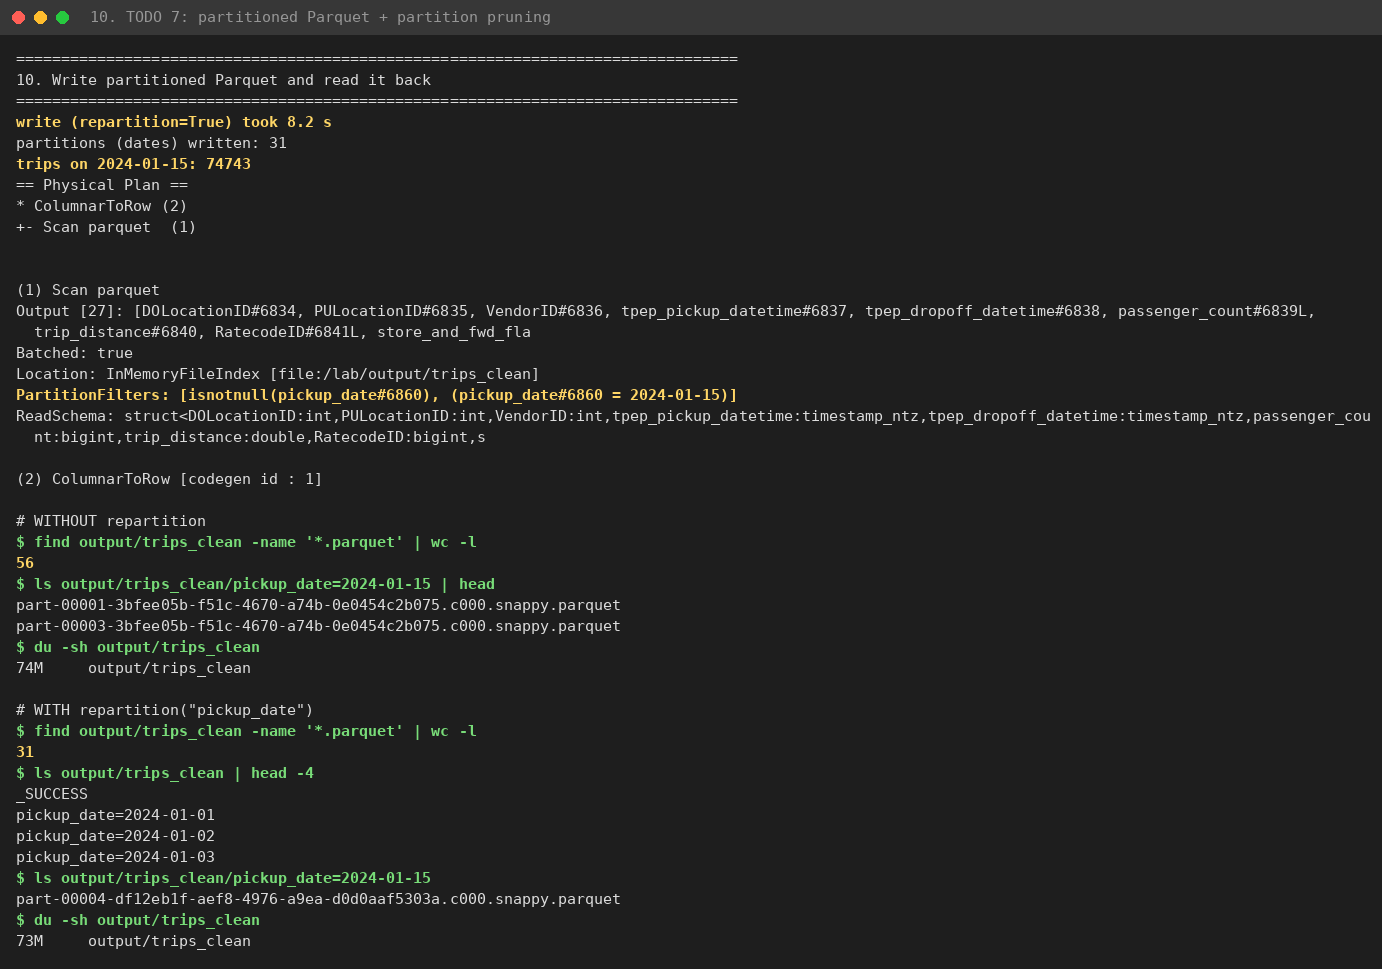
\includegraphics[keepaspectratio]{img/07_write_partitioned_pruning.png}}
\caption{write + pruning}
\end{figure}

Không \texttt{repartition}, mỗi task trong 4 task ghi một file cho
\textbf{mỗi ngày mà nó chứa}. Ở đây chỉ ra 56 file chứ không phải 4 × 31
= 124, vì file nguồn gần như đã sắp theo thời gian: mỗi task chỉ chứa
một khoảng ngày liền nhau, và các ngày ở ranh giới bị tách thành 2 file.
Với dữ liệu không có thứ tự và hàng trăm task, số file sẽ là N × 31. Khi
đọc lại,
\texttt{PartitionFilters:\ {[}isnotnull(pickup\_date),\ (pickup\_date\ =\ 2024-01-15){]}}
cho thấy Spark chỉ mở \textbf{một thư mục}.

\subsection{Trả lời checkpoint}\label{trux1ea3-lux1eddi-checkpoint}

\textbf{Q1.} Spark chia file thành input partition dựa trên: -
\texttt{spark.sql.files.maxPartitionBytes}, mặc định 128 MB; - mục tiêu
có ít nhất \texttt{defaultParallelism} split (= 4 core với
\texttt{local{[}4{]}}), nên kích thước split được hạ xuống khoảng 48 MB
/ 4.

Parquet chỉ cắt được ở ranh giới \textbf{row group}: task nào nhận được
điểm bắt đầu của row group thì đọc row group đó. Vì vậy dù chỉ có một
file 48 MB vẫn ra \textbf{4 partition}, và một partition có thể rỗng nếu
số row group ít hơn 4.

\textbf{Q2.} \texttt{filter}, \texttt{withColumn} và \texttt{select} là
\textbf{transformation}: chúng chỉ thêm node vào logical plan, không
đụng tới dữ liệu, nên mất 0.096 s. \texttt{count()} là \textbf{action}:
Catalyst tối ưu plan, DAG scheduler tạo stage và task, rồi mới đọc file
(0.28 s). \texttt{show}, \texttt{collect}, \texttt{take}, \texttt{write}
và \texttt{count} cũng là action. Plan dựng trong vài mili-giây vì đó
chỉ là thao tác trên cây biểu thức trong bộ nhớ của driver.

\textbf{Q3 (lazy evaluation và DAG).} \texttt{by\_borough.show()} là SQL
query 10. Nó sinh ra \textbf{4 job} (19--22) với AQE:

\begin{longtable}[]{@{}
  >{\raggedright\arraybackslash}p{(\linewidth - 6\tabcolsep) * \real{0.2500}}
  >{\raggedright\arraybackslash}p{(\linewidth - 6\tabcolsep) * \real{0.2500}}
  >{\raggedright\arraybackslash}p{(\linewidth - 6\tabcolsep) * \real{0.2500}}
  >{\raggedright\arraybackslash}p{(\linewidth - 6\tabcolsep) * \real{0.2500}}@{}}
\toprule\noalign{}
\begin{minipage}[b]{\linewidth}\raggedright
Job
\end{minipage} & \begin{minipage}[b]{\linewidth}\raggedright
Stage
\end{minipage} & \begin{minipage}[b]{\linewidth}\raggedright
Số task
\end{minipage} & \begin{minipage}[b]{\linewidth}\raggedright
Việc làm
\end{minipage} \\
\midrule\noalign{}
\endhead
\bottomrule\noalign{}
\endlastfoot
19 & 25 & 1 & dựng broadcast bảng zone cho \textbf{pickup}
(\texttt{BroadcastExchange}) \\
20 & 26 & 1 & dựng broadcast bảng zone cho \textbf{dropoff} \\
21 & 27 & \textbf{4} & đọc \texttt{InMemoryTableScan} (cache), 2 ×
\texttt{BroadcastHashJoin}, \texttt{HashAggregate} partial, \textbf{ghi
shuffle} (\texttt{Exchange\ hashpartitioning(pu\_borough,\ 8)}) \\
22 & 28 (skipped, dùng lại output của 27), \textbf{29} & 1 &
\texttt{AQEShuffleRead\ coalesced} (8 → 1 partition),
\texttt{HashAggregate} final, \texttt{TakeOrderedAndProject} cho
\texttt{orderBy\ +\ show} \\
\end{longtable}

\begin{itemize}
\tightlist
\item
  \textbf{Ranh giới stage là các toán tử \texttt{Exchange} (shuffle).}
\item
  Broadcast chạy thành job riêng.
\item
  Với AQE, mỗi query stage được nộp thành một job riêng, nên stage của
  job trước hiện là \emph{skipped} trong job sau.
\item
  Khi chạy toàn bộ \texttt{by\_borough} (ví dụ \texttt{collect}), plan
  còn có \texttt{Exchange\ rangepartitioning(trips\ DESC,\ 8)} cho
  \texttt{orderBy}, tức là thêm một stage sort nữa (xem
  \texttt{explain}).
\item
  Không có gì chạy cho tới khi gọi \texttt{show()}. Các transformation ở
  mục 4--5 chỉ dựng DAG.
\end{itemize}

\textbf{Q4.} 5 cột có cùng 140,162 NULL vì đó là \textbf{cùng 140,162
chuyến}. Các bản ghi này được gửi lên thiếu toàn bộ nhóm trường
``metadata'' (thường từ một vendor hoặc từ chuyến street-hail), chứ
không phải 5 lỗi độc lập. Có ba cách xử lý: - giữ lại và gán mặc định,
như script làm: \texttt{passenger\_count=1}, \texttt{RatecodeID=1}, phụ
phí = 0; - giữ NULL và chỉ loại khỏi các chỉ số cần những cột đó; - tách
ra vùng quarantine.

Cách nào cũng cần thống nhất với chủ dữ liệu và ghi lại trong tài liệu.

\textbf{Q5 (đọc formatted plan).} Đọc từ dưới lên: 1.
\texttt{Scan\ parquet} với \texttt{PushedFilters}
(\texttt{GreaterThan(fare\_amount,0.0)},
\texttt{LessThanOrEqual(trip\_distance,100.0)}\ldots): luật làm sạch
được đẩy xuống reader Parquet. 2. \texttt{InMemoryTableScan}: đọc từ
cache. 3. 2 × \texttt{BroadcastExchange} và
\texttt{BroadcastHashJoin\ LeftOuter\ BuildRight}. 4.
\texttt{HashAggregate} (22) với
\texttt{partial\_count(1),\ partial\_avg(...)}. Mỗi task \textbf{gộp
trước} các dòng của nó theo \texttt{pu\_borough}. \texttt{avg} được tách
thành cặp \texttt{(sum,\ count)}, nên mỗi task chỉ phát ra khoảng 6--8
dòng; tổng cộng \textbf{24 dòng} đi qua shuffle thay vì 2.87 triệu. 5.
\texttt{Exchange\ hashpartitioning(pu\_borough,\ 8)}: \textbf{shuffle},
cũng là ranh giới stage. 6. \texttt{AQEShuffleRead\ coalesced}: AQE gộp
8 partition shuffle nhỏ lại. 7. \texttt{HashAggregate} (26) final với
\texttt{count(1),\ avg(...)}: gộp các kết quả partial. 8.
\texttt{Exchange\ rangepartitioning} và \texttt{Sort} cho
\texttt{orderBy}.

Partial/final aggregate chính là \textbf{combiner của L02}. Tách
\texttt{avg} thành \texttt{(sum,\ count)} cũng giống hệt cách làm ở bài
stretch L02 (combiner tính giá cước trung bình).

\textbf{Q6.} Bảng zone chỉ có 265 dòng (12 KB, khoảng 1 MB trong bộ nhớ
theo \texttt{Statistics(sizeInBytes=1026.1\ KiB)}), nhỏ hơn nhiều so với
\texttt{spark.sql.autoBroadcastJoinThreshold} (10 MB). Spark gửi một bản
sao cho mọi task, nên 2.87 triệu chuyến \textbf{không phải shuffle}. Khi
cả hai bên đều lớn hơn ngưỡng (hoặc đặt ngưỡng = -1, hoặc thống kê kích
thước vượt ngưỡng), Spark shuffle cả hai bên theo key và dùng
\textbf{SortMergeJoin}. L06 đo sự khác biệt này.

\textbf{Q7.} Sau khi \texttt{cache()}: - \textbf{Plan} đọc từ
\texttt{InMemoryRelation}/\texttt{InMemoryTableScan} thay vì quét và lọc
lại Parquet. - \textbf{Tab Storage} hiện RDD đã cache: 4 partition, 100
\%, 347.3 MiB. - Các action sau nhanh hơn, ví dụ \texttt{clean.count()}
lần đầu (materialize cache) mất khoảng 6 s, còn các query sau chỉ
0.3--1.5 s.

Cache là ý tồi khi: - dữ liệu chỉ dùng một lần; - dữ liệu không vừa bộ
nhớ, gây spill, eviction và áp lực GC (347 MiB cache so với 48 MB
Parquet nén là hệ số khoảng 7×); - đọc nguồn vốn đã rẻ (Parquet có
column pruning có thể nhanh hơn cache dạng hàng rộng); - quên
\texttt{unpersist()}, làm giữ bộ nhớ không cần thiết.

\textbf{Q8.} \texttt{partitionBy} ghi \textbf{một file cho mỗi task ×
mỗi giá trị partition} mà task đó chứa. Không \texttt{repartition}, mỗi
task có thể chứa dòng của nhiều ngày, và số file có thể lên tới N task ×
31 ngày. Ở đây đo được 56 file; trên cluster thật sẽ là hàng nghìn file
nhỏ, gây hại cho NameNode và cho tốc độ đọc.
\texttt{repartition("pickup\_date")} shuffle trước để mọi dòng của một
ngày về cùng một task, nên ra \textbf{đúng 1 file/ngày (31 file)}. Cái
giá là thêm một shuffle (6.8 s → 8.2 s). Cần cẩn thận khi một giá trị
quá lớn (skew): một task sẽ phải ghi cả file khổng lồ. Khi đó dùng
\texttt{repartition(n,\ "pickup\_date",\ salt)} hoặc
\texttt{maxRecordsPerFile}.

\end{document}
